%%%%%%%%%%%%%%%%%%%%%%%%%%%%%%%%%%%%%%%%%%%%%%%%%%%%%%%%%%%%
%%% LIVECOMS ARTICLE TEMPLATE FOR BEST PRACTICES GUIDE
%%% ADAPTED FROM ELIFE ARTICLE TEMPLATE (8/10/2017)
%%%%%%%%%%%%%%%%%%%%%%%%%%%%%%%%%%%%%%%%%%%%%%%%%%%%%%%%%%%%
%%% PREAMBLE
\documentclass[9pt,tutorial,ASAPversion]{livecoms}

% Use the 'onehalfspacing' option for 1.5 line spacing
% Use the 'doublespacing' option for 2.0 line spacing
% Use the 'lineno' option for adding line numbers.
% Use the "ASAPversion' option following article acceptance to add the DOI and relevant dates to the document footer.
% Use the 'pubversion' option for adding the citation and publication information to the document footer, when the LiveCoMS issue is finalized.
% The 'bestpractices' option for indicates that this is a best practices guide.
% Omit the bestpractices option to remove the marking as a LiveCoMS paper.
% Please note that these options may affect formatting.

\usepackage{lipsum} % Required to insert dummy text
\usepackage[version=4]{mhchem}
\usepackage{siunitx}
\usepackage{subcaption}
\usepackage{graphicx}
\usepackage{tabu}
\usepackage{color}
\usepackage{outlines}
\DeclareSIUnit\Molar{M}
\usepackage[italic]{mathastext}
\graphicspath{{figures/}}

%%%%%%%%%%%%%%%%%%%%%%%%%%%%%%%%%%%%%%%%%%%%%%%%%%%%%%%%%%%%
%%% IMPORTANT USER CONFIGURATION
%%%%%%%%%%%%%%%%%%%%%%%%%%%%%%%%%%%%%%%%%%%%%%%%%%%%%%%%%%%%

\newcommand{\versionnumber}{1.0}  % you should update the minor version number in preprints and major version number of submissions.
\newcommand{\githubrepository}{\url{https://github.com/westpa/westpa_tutorials}}  %this should be the main github repository for this article

%%%%%%%%%%%%%%%%%%%%%%%%%%%%%%%%%%%%%%%%%%%%%%%%%%%%%%%%%%%%
%%% ARTICLE SETUP
%%%%%%%%%%%%%%%%%%%%%%%%%%%%%%%%%%%%%%%%%%%%%%%%%%%%%%%%%%%%
\title{A Suite of Tutorials for the WESTPA Rare-Events Sampling Software [Article v\versionnumber]}

\author[1*]{Anthony T. Bogetti}
\author[2*]{Barmak Mostofian}
\author[3*]{Alex Dickson}
\author[1*]{AJ Pratt}
\author[1*]{\\ Ali S. Saglam}
\author[1*]{Page O. Harrison}
\author[4]{Joshua L. Adelman}
\author[1]{Max Dudek}
\author[1]{\\Paul A. Torrillo}
\author[1,5]{Alex J. DeGrave}
\author[2,6]{Upendra Adhikari}
\author[7]{Matthew C. Zwier}
\author[2]{Daniel M. Zuckerman}
\author[1]{and Lillian T. Chong}
\affil[1]{Department of Chemistry, University of Pittsburgh, Pittsburgh, PA}
\affil[2]{Department of Biomedical Engineering, Oregon Health and Science University, Portland, OR}
\affil[3]{Department of Biochemistry and Molecular Biology, Michigan State University, East Lansing, MI}
\affil[4]{Department of Biological Sciences, University of Pittsburgh, Pittsburgh, PA; currently unaffiliated}
\affil[5]{Current address: Paul G. Allen School of Computer Science and Engineering, University of Washington, Seattle, WA}

\affil[6]{Current address: Department of Chemistry, Missouri Valley College, Marshall, MO}
\affil[7]{Department of Chemistry, Drake University, Des Moines, IA}

\corr{ltchong@pitt.edu}{LTC}  % Correspondence emails.  FMS and FS are the appropriate authors initials.
\corr{zuckermd@ohsu.edu}{DMZ}  % Correspondence emails.  FMS and FS are the appropriate authors initials.

%\orcid{Author 1 name}{AAAA-BBBB-CCCC-DDDD}
%\orcid{Author 2 name}{EEEE-FFFF-GGGG-HHHH}

\contrib[*]{These authors contributed equally to this work}

%\presentadd[\authfn{3}]{Department, Institute, Country}
%\presentadd[\authfn{4}]{Department, Institute, Country}

\blurb{This LiveCoMS document is maintained online on GitHub at \githubrepository; to provide feedback, suggestions, or help improve it, please visit the GitHub repository and participate via the issue tracker.}

%%%%%%%%%%%%%%%%%%%%%%%%%%%%%%%%%%%%%%%%%%%%%%%%%%%%%%%%%%%%
%%% PUBLICATION INFORMATION
%%% Fill out these parameters when available
%%% These are used when the "pubversion" option is invoked
%%%%%%%%%%%%%%%%%%%%%%%%%%%%%%%%%%%%%%%%%%%%%%%%%%%%%%%%%%%%
\pubDOI{10.XXXX/YYYYYYY}
\pubvolume{<volume>}
\pubissue{<issue>}
\pubyear{<year>}
\articlenum{<number>}
\datereceived{18 June 2019}
\dateaccepted{26 September 2019}

%%%%%%%%%%%%%%%%%%%%%%%%%%%%%%%%%%%%%%%%%%%%%%%%%%%%%%%%%%%%
%%% ARTICLE START
%%%%%%%%%%%%%%%%%%%%%%%%%%%%%%%%%%%%%%%%%%%%%%%%%%%%%%%%%%%%

\begin{document}

\begin{frontmatter}
\maketitle

\begin{abstract}
The weighted ensemble (WE) strategy has been demonstrated to be highly efficient in generating pathways and rate constants for rare events such as protein folding and protein binding using atomistic molecular dynamics simulations. 
Here we present five tutorials instructing users in the best practices for preparing, carrying out, and analyzing WE simulations for various applications using the WESTPA software. 
Users are expected to already have significant experience with running standard molecular dynamics simulations using the underlying dynamics engine of interest (e.g. Amber, Gromacs, OpenMM). 
The tutorials range from a molecular association process in explicit solvent to more complex processes such as host-guest association, peptide conformational sampling, and protein folding. 
\end{abstract}

\end{frontmatter}

\section{Introduction and Scope of Tutorials}

WESTPA (The Weighted Ensemble Simulation Toolkit with Parallelization and Analysis; \url{https://westpa.github.io/westpa}) \citep{Zwier2015} is an open-source, highly scalable software framework for carrying out extended-timescale simulations of rare events with rigorous kinetics using the weighted ensemble (WE) strategy \citep{HuberKim1996}. 
Key features of WESTPA, written in Python, include (i) a general interface that enables interoperability with any dynamics engine (e.g. Gromacs \citep{gromacs}, Amber \citep{amber}, OpenMM \citep{openmm}); (ii) an optimized, parallel implementation of the WE strategy that exhibits perfect scaling out to >4000 CPU cores ; (iii) an effective suite of tools for analysis of the millions of files created by each simulation; (iv) full extensibility for enhancements to simulation protocols and analysis tools; and (v) portability of the software on any Unix-like computing resource, including typical computing clusters and supercomputers. 
The WESTPA software also includes plugins for using a WE-based string method \citep{Adelman2013} and a WE strategy utilizing hierarchical Voronoi bins (WExplore) \citep{Dickson2014}.  
The WESTPA software package has enabled efficient atomistic simulations of host-guest associations \citep{Zwier2011}, protein binding processes \citep{Zwier2016, Saglam2019}, and protein folding \citep{Upendra2019}. 
This efficiency (relative to standard “brute force” simulations) has been demonstrated to increase exponentially with the effective free energy barrier of the rare event \citep{DeGrave2018}. 

Here we present a suite of five tutorials for the WESTPA software in order of difficulty from basic to advanced, including a tutorial involving the suite of analysis tools. These tutorials can also be found online in our WESTPA GitHub repository (\url{https://github.com/westpa/westpa_tutorials/wiki})
Learning objectives and expected outcomes are outlined for each tutorial. 
This set of tutorials is restricted to applications in molecular dynamics (MD) simulations, but WE and WESTPA are applicable to arbitrary stochastic simulations \citep{Donovan2013,Donovan2016,Read2018}.

After completing the Basic Tutorial involving the simulation of Na\textsuperscript{+}/Cl\textsuperscript{-} association, the user should be able to: 
\begin{enumerate}
\item Understand the main simulation directory layout
\item Choose a progress coordinate
\item Choose an appropriate binning scheme
\item Prepare input files
\item Monitor a simulation
\end{enumerate}

After completing the Intermediate Tutorial involving the conformation sampling of a p53 peptide fragment, the user should be able to:
\begin{enumerate}
\item Set up a two-dimensional progress coordinate
\item Monitor this coordinate as the simulation progresses
\item Evaluate whether the binning scheme is effective
\item Combine and create bins “on-the-fly”
\item Store and access auxiliary data
\end{enumerate}

After completing Advanced Tutorial 1 involving the folding/unfolding of the chignolin mini-protein the user should be able to:
\begin{enumerate}
\item Use brute force simulations to identify appropriate initial and/or a target states
\item Obtain the probability flux into the target state of a WESTPA simulation, how to convert it to a mean rate constant, and how to interpret the results
\item Approach larger, more biologically relevant events (like protein folding) with a WE-oriented mindset
\end{enumerate}

After completing Advanced Tutorial 2 involving K\textsuperscript{+}/18-crown-6 ether association and WExplore plugin, the user should be able to:
\begin{enumerate}
\item Install and use the WExplore-WESTPA plugin
\item Define and implement their own distance metric for use in WExplore simulation
\item Determine appropriate values for WExplore-specific parameters for their system of interest
\item Analyze simulations by inspecting properties of the Voronoi “images” 
\end{enumerate}

After completing the Analysis Tutorials, the user should be able to:
\begin{enumerate}
\item Calculate progress coordinates using an external analysis suite (MDTraj or MDAnalysis)
\item Automate analysis and interactively explore WE simulation data using the w\textunderscore \verb|ipa| tool
\item Create a movie of how a probability distribution evolves with time
\end{enumerate}

The tutorials will use an array of different dynamics packages to showcase WESTPA’s interoperability. All of these packages and the auxiliary programs required (for analysis etc.) for each tutorial are freely available and documentation can readily be found online.  The versions of each software package used is also provided in each tutorial’s “computational requirements” section. 

\subsection{Using WE Concepts in MD Simulation}

The WE strategy organizes an array of MD trajectories strategically in configuration space to target quantities of interest which would not be calculable via standard MD. 
Typical examples are the calculation of pathways and rate constants for conformational and binding processes. 
The overall WE strategy can be embodied in a wide variety of specific algorithms. 
The WESTPA software can be considered a direct descendent of the Huber and Kim algorithm \citep{HuberKim1996}, although the idea to use trajectory “splitting” and reweighting had been devised decades earlier for research at Los Alamos \citep{KahnHarris1951}.  

As sketched in Figure 1, the essence of WE is to use a statistically unbiased, weighted sample of MD trajectories in such a way that a higher density of trajectories is deployed in regions of configuration space where sampling would otherwise be rare in standard MD. 
These rare regions might be (free) energetic barriers or merely distant regions of configuration space. 
The trajectory weights, which are fundamental to WE, result from the statistical resampling procedures which either prune or replicate trajectories according to rules implemented in WESTPA \citep{HuberKim1996,Zhang2010,Zwier2015}. 
The rules typically generate trajectory replicates---which will diverge upon additional simulation using a stochastic thermostat or dynamics---in under-sampled regions while pruning trajectories that occur in over-sampled regions.  

Procedurally, WE runs a large number of ordinary, unbiased MD trajectory segments in parallel, with each segment halted and examined after a short interval of time (e.g. 1-100 ps, see Table 1) called $\tau$. 
After each interval, some trajectories are replicated and some are pruned according to user-specified parameters - see below. 
This in turn triggers automated adjustment of the weights to complete the resampling process. 
The remaining trajectories are then continued for another $\tau$ interval.

%%%Fig 1%%%
\begin{figure}
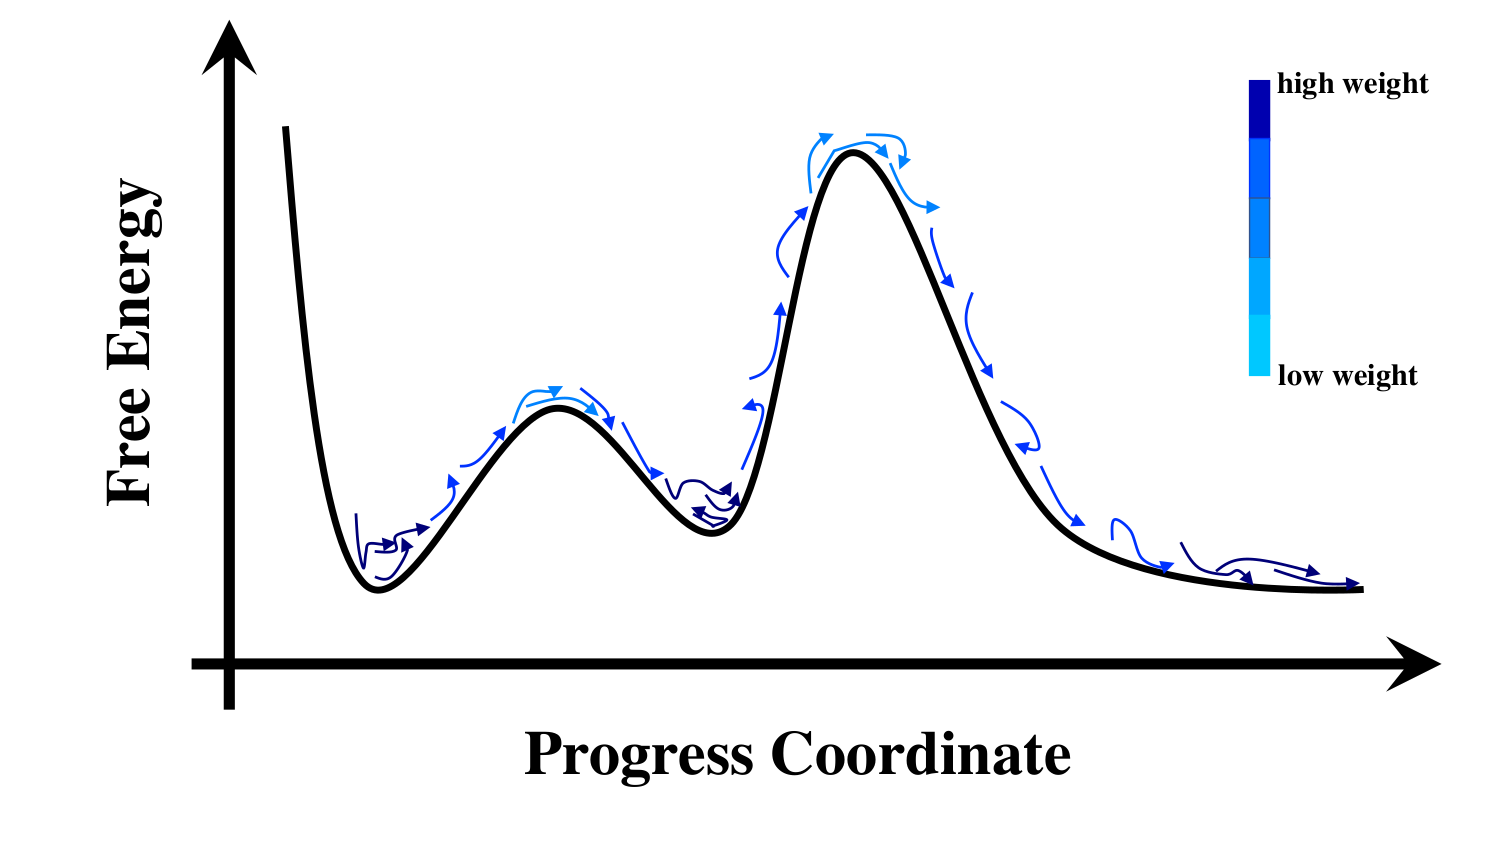
\includegraphics[width=\linewidth]{Figure1.png}
\caption{Weighted ensemble MD simulations. 
Trajectory segments (blue) are fairly evenly distributed in configuration space, and hence enhance sampling of normally undersampled regions of configuration space, such as free energy barriers. 
In this schematic, the free energy or potential of mean force is shown as a function of an arbitrary progress coordinate.
Darker color denotes higher weight trajectories, which will occur at free energy minima and regions initially seeded with trajectories and probability.}
\label{fig:view}
\end{figure}
%%%%%%%%

The rules for resampling trajectories without bias are extremely flexible \citep{Zhang2010} and numerous possibilities are implemented within the WESTPA software. 
Typically, WE simulations rely on “bins,” which are defined regions of configuration space for which the user defines a target number of trajectories \citep{HuberKim1996}. 
In WESTPA, bins can be constructed from simple one or two-dimensional “progress coordinates”, a hierarchical nesting of bins inside of other bins, Voronoi cells, or the WExplore hierarchical Voronoi strategy \citep{Zwier2015,Dickson2014}.
Strictly speaking, it is worth noting that bins are not required to perform WE-like resampling \citep{Dickson2018or19}.

Each WE simulation ultimately yields an ensemble of trajectories, from which different types of information can be extracted. 
Each trajectory which makes a full transition between states of interest, say from A to B, yields an ordered set of configurations which can be analyzed for structural changes and the sequence of events. 
The full weighted ensemble of trajectories, if clustered into pathway groups, can provide information on the relative importance of different pathways \citep{Ernesto2019}. 
If WE was performed with a “recycling” condition where trajectories reaching B are fed back to A, then the rate constant for the process can be estimated from the probability flux arriving to state B if the simulation achieves steady state and hence constant flux \citep{Divesh2010,ZuckermanChong2017}.
If a WE simulation does not achieve steady state, it is still possible in principle to estimate rate constants using a non-Markovian analysis, also called a history-augmented Markov State Model \cite{Ernesto2014,Upendra2019,Jeremy2019}.

\subsection{Prerequisites}

\subsubsection{Background Knowledge and Experience}

The WESTPA software is not intended for total beginners in molecular simulation. 
A prerequisite for all of WESTPA tutorials presented here is that users already have extensive experience with running standard molecular dynamics (MD) simulations using the underlying dynamics engine of interest (Amber, Gromacs, OpenMM, etc.). 
In fact, we recommend running multiple short, standard simulations prior to applying the WE strategy in order to (i) ensure that the system is prepared and the dynamics are propagated according to best practices (e.g., see \citep{Mobley2019}), (ii) identify potential progress coordinates and other observables that may be worth monitoring during the WE simulation, (iii) determine an initial definition of the target state, and (iv) estimate storage needs for your eventual WE simulation and the ns/day that can be generated for your system. 
It is also important to identify sources of validation for your simulation (e.g., from experiment and/or standard simulations) and to be familiar with the estimation of statistical uncertainty in the computed observables, including those used for validation (\citep{Grossfield2019}). 
We highly recommend that new users read the WE overview (\url{https://www.csb.pitt.edu/Faculty/zuckerman/we-overview.pdf}) as well as a recent review article \citep{ZuckermanChong2017}. 
In addition, new users are encouraged to search the WESTPA mailing list (\url{https://groups.google.com/forum/#!forum/westpa-users}) for possible solutions or submit questions/issues there.

\subsubsection{Software Requirements}

The WESTPA software requires Python and a number of standard Python scientific computing packages. 
All required software is available through the Anaconda Python distribution, which also provides the preferred mechanism for obtaining and installing WESTPA itself. 
The software can be used on any Unix operating system, including academic clusters and supercomputers. 
The installation of WESTPA is streamlined by an Anaconda conda install recipe that enables WESTPA and all software dependencies to be installed at the same time.

In addition, WESTPA will require interfacing with an external dynamics engine in order to run WE simulations.  Examples of dynamics engines that can be used (all free of charge), and the versions used are included before each tutorial in this manuscript.

\subsubsection{Hardware Requirements}

The highly scalable WESTPA software is particularly well-suited for high-performance computing (HPC) clusters, including those at academic institutions or supercomputing centers. 
Much of the computing effort is independent (i.e. highly parallelizable) with only a small amount of data being transferred to a central process at the end of each WE iteration. 
Furthermore, the amount of memory per computing node need only be sufficient for the underlying dynamics engine, e.g., \textasciitilde 1 GB per CPU core for atomistic MD simulations. 

The two major computing hardware requirements for large-scale WESTPA simulations are (i) the number of available processors, and (ii) the amount of disk storage in the scratch (working) space. 
Further details about these requirements are provided below. 

\textbf{Number of Processors.} WESTPA can be run on even a single processor, but the ideal scenario is to use the same number of processors — all with the same processor speed — as the number of trajectories you are simultaneously running at any point in time; in this way, all trajectories that are being run can be completed at the same time. 
If the ideal number of processors is not available, we suggest requesting a number by which the number of trajectories at any point in time is divisible. 
These are not strict requirements, but following these guidelines will ensure the most economical use of computer time possible.

\textbf{Storage Requirements.} To estimate the storage requirement for your WE simulation, we suggest running a single MD simulation for length $\tau$, estimating the maximum number of trajectories you will generate for any WE iteration (number of bins multiplied by number of trajectories per bin), and estimating the number of WE iterations you will need to converge the observable of interest. 
This results in the maximum total number of trajectories per simulation, which can be used to estimate the total storage requirements (both number of files and aggregate storage space). 
Ideally, the scratch space of your computing cluster should be sufficiently large to temporarily store the entire simulation, which makes the analysis easier in the not-unlikely event you need to reanalyze each trajectory. 
Regardless of your estimate, having an off-cluster storage option that can store the simulation in case you need to extend the simulation further on the cluster would be ideal. 
Also, make sure that you are not exceeding any limits on the total number of files a user can have on your computing cluster. 

As an example, we present the hardware requirements of our largest-scale WESTPA simulation to date, which involved a protein-protein binding process in explicit solvent. 
To enable convenient analysis of this simulation, the scratch directory of a computing cluster would ideally allow for 15 TB of disk space to store trajectory coordinates for the entire system, including explicit water molecules, checkpoint files for continuing trajectories, and other files required for analysis. 
If the scratch space is much less than this amount (e.g. 2 TB), we recommend separately tarring and archiving each WE iteration, keeping the last five WE iterations untarred, and moving the archived files to local storage. 
This strategy enables one to restart a WE simulation from the last few iterations if necessary. 
We realize that this protein-protein binding simulation is an extreme use case, but nonetheless, this scenario highlights the importance of allocating the necessary storage space for more typical use cases. 

We note that most distributed storage filesystems used on large clusters (e.g. Lustre or GPFS) do not distribute metadata (file size, modification time, etc.) processing, and this centralized treatment of metadata can become a "choke point" for WESTPA simulations. 
In the worst case, a poorly-configured WESTPA simulation can result in denial of service to other users. 
There are no viable alternative file systems at this time. 
Fortunately, a simple remedy exists. The burden of running WESTPA simulations on these distributed filesystems can be substantially reduced by using the full pathnames to all executables called by any WESTPA process (for example, writing \verb|/usr/bin/awk| instead of simply \verb|awk|).

\subsubsection{Running WESTPA on a Computing Cluster}

Prior to running full-blown WESTPA simulations on your desired computing cluster, it is advisable to consult with the system administrator about how best to run your simulation on the cluster. 
In addition, test simulations consisting of a few WE iterations should be run using the development queue to gauge if the I/O is too frequent for the cluster and to optimize the execution of your simulation (see Table 1 for examples of computing resources that have been suitable for various WE applications). 
Sample shell scripts for executing WESTPA simulations on various computing resources have been provided for the Intermediate Tutorial (Section 6.2) on GitHub. 

\begin{table*}
\caption{WE parameters used for notable applications in the literature. 
The asterisk (*) indicates an application with I/O operations that is too frequent for supercomputers and gaming GPUs.}
\centering
\begin{tabular}{ | p{0.22\linewidth} | p{0.22\linewidth} | p{0.22\linewidth} | p{0.22\linewidth} |}
\hline
\textbf{Rare-event process} & 
\textbf{System and size} & 
\textbf{WE Parameters} & 
\textbf{Suitable computing resources} \\
\hline
millisecond protein folding \citep{Mostofian2019} & 
NTL9 protein in generalized Born (GB) implicit solvent with low and high solvent viscosity (collision frequency of 5 ps\textsuperscript{-1} and 80 ps\textsuperscript{-1}, respectively) 627 atoms & 
1D progress coordinate: C\textsubscript{$\alpha$} RMSD from the folded structure

Binning: 53 bins, that are finely spaced for near-folded structures (35 bins for 1.0 \AA{} < RMSD < 4.4 \AA) and more coarsely spaced for more unfolded structures (12 bins for 4.4 \AA{} < RMSD < 6.6 \AA; 5 bins for 6.6 \AA < RMSD < 10.2 \AA)

$\tau$ = 10 ps 

1,200 WE iterations

4 trajectories/bin
& Professional-Graphics-programming GPUs\textsuperscript{*} (e.g. NVIDIA GTX 1080) \\
\hline
peptide-protein association \citep{Zwier2016} & 
p53 peptide and MDM2 protein in GB/SA implicit solvent: 1685 atoms & 
2D progress coordinate: heavy-atom RMSD of p53 peptide relative to its MDM2-bound conformation following alignment on (i) MDM2 and (ii) itself. 

Binning: 16 bins with 0.5 \AA{} widths along the p53-aligned RMSD and widths ranging from 0.2 to 2 \AA{} for the MDM2-aligned RMSD. 

$\tau$ = 50 ps; 396 WE iterations
8 trajectories/bin & 
1600 CPU cores on a supercomputer (e.g. XSEDE’s Bridges) or 16 GPUs (e.g. NVIDIA Tesla P100 GPUs) \\
\hline
protein-protein association \citep{Saglam2019} & 
barnase and barstar proteins in explicit solvent: >100,000 atoms & 
2D progress coordinate: (i) heavy-atom RMSD of barstar residues D35 and D39 after alignment on barnase, and (ii) minimum protein-protein separation distance.  
D35 and D39 are the barstar residues that become the most buried upon binding barnase.

$\tau$ = 20 ps; 650 WE iterations

Binning: 72 bins with coarsely spaced bins every 1 \AA{} from 10 to 60 \AA{} and more finely spaced bins every 0.5 \AA{} from 0 to 10 \AA{} along the RMSD coordinate; two bins along the distance coordinate separated by a bin boundary at 5 \AA{}. & 
1600 CPU cores on a supercomputer (e.g. XSEDE’s Bridges) or 16 GPUs (e.g. NVIDIA Tesla P100 GPUs) \\
\hline
\end{tabular}
\end{table*}

\section{Workflow of Running a WE Simulation}

An overview of the workflow for running a WE simulation using WESTPA is detailed below. 
This workflow is only meant to give a sense of the mechanics and flow of using WESTPA once your system and WE parameters have already been carefully chosen. See Table 2 for a summary of all files mentioned in this workflow.

\begin{table}
\caption{WEST\_SIM\_ROOT organization and file explanations}
\centering
\begin{tabular}{| r | l |}
\hline
\verb|bstates/| & directory containing basis states \\
\hline
\verb|env.sh| & set environment variables \\
\hline
\verb|init.sh| & initialize the WESTPA simulation \\
\hline
\verb|common_files/| & directory containing files for \\
{} & dynamics (i.e. topologies) \\
\hline
\verb|run.sh| & run the WESTPA simulation \\
\hline
\verb|tstate.file| & define the target state (for steady state \\
{} & simulations only) \\
\hline
\verb|west.cfg| & specify most WE simulation parameters \\
\hline
\verb|westpa_scripts/| & directory containing essential scripts \\
\hline
\verb|system.py| & a separate script to define functions or \\
{} & parameters (optional) \\
\hline
\verb|reference/| & directory containing reference files for \\
{} & calculations (optional) \\
\hline
\end{tabular}
\end{table}

\textbf{Overall Flow}

\textbf{Ready:} The purpose of this step is to ensure that the chosen WE parameters are correctly specified in the proper places and that all environment variables are correctly set. 
Most of the WE parameters (such as the number of WE iterations, binning scheme etc.) and auxiliary datasets (auxdata; see Section 6.2) are specified in the \verb|west.cfg| file. 
You can view an example of this file in any of the tutorials below; labels exist directing where to specify each parameter. 
More complex binning schemes (such as recursive schemes or schemes involving functional bin mappers) can be specified in an external file called \verb|system.py|. 
A user may also choose to write functions to this file. 
Usually, these functions will calculate progress coordinate or auxiliary data and are more complex than usual.

The environment is set up in the \verb|env.sh| file. 
The location of the main WESTPA simulation directory (\verb|WEST_SIM_ROOT|) and the location of dynamics/analysis programs are placed in your system path. 
When setting up WESTPA on a cluster, program modules will be loaded in the \verb|runwe.slurm| file instead of the \verb|env.sh| file (see Section 6.1 and view the cluster-specific \verb|runwe.slurm| file). 
It is a best practice to define variables in \verb|env.sh| for each program that will be called. 
These variables should contain the full path to that program (such as \verb|CPPTRAJ=$(which cpptraj|), see Section 4.3 for more information). 
Always source \verb|env.sh| before trying to run WESTPA just to see if any errors appear relating to programs not being found. 
If errors are present, edit \verb|env.sh| to specify the proper locations of programs and try to source it again. 
The goal of this action is to make sure that any issues with your environment are fixed before continuing so that troubleshooting becomes much easier later on. 

\textbf{Set:} After setting up the system environment and specifying the WE parameters, users will need to initialize the simulation. 
This involves running the \verb|init.sh| script, which will take an initial structure (or structures), calculate a progress coordinate (pcoord for short, this is also the name used in WESTPA datasets pertaining to the progress coordinate) value for that structure and then place that structure in the appropriate bin. 
The \verb|init.sh| file is also the location where users can specify whether the simulation will be run under equilibrium or steady-state conditions. 

Place the starting structure(s) in the \verb|bstates/| directory. 
The structure should be a coordinate file giving the starting configuration of your system (e.g. Amber restart file). 
The \verb|bstate.file| tells WESTPA which structure to use as the initial structure for the simulation. 
If you have only one structure, this file will contain the name of that structure only; if you have more than one structure, \verb|bstate.file| should list each structure along with its associated statistical weight. 
An example of the latter is a representative ensemble of unbound protein conformations in a binding process that could be generated using a prior equilibrium WE simulation \citep{Zwier2016,Saglam2019}. 

Next, specify whether the simulation will be run under equilibrium or steady-state conditions. 
This specification is made in the \verb|init.sh| file. 
Including a \verb|TSTATE_ARGS| argument for \verb|w_init| will signal for WESTPA to run under steady state conditions. 
The \verb|tstate.txt| file in the main simulation directory is where the progress coordinate value of the target state is specified. 
If the \verb|TSTATE_ARGS| argument is absent, the simulation will be run under equilibrium conditions. 
See the tutorials in Sections 6.1 and 6.2 below for examples of how \verb|init.sh| will change from running a steady-state simulation versus an equilibrium simulation (respectively).

Running \verb|init.sh| will cause WESTPA to execute \verb|get_pcoord.sh|, which is a script located in \verb|westpa_scripts/|. 
This script will give an initial progress-coordinate value for the basis state(s) (located in \verb|bstates/|) to WESTPA.


Users will need to modify \verb|get_pcoord.sh| to either read or calculate the progress coordinate for their particular simulation.
For instance, in the Basic Tutorial, the distance between the Na\textsuperscript{+} and Cl\textsuperscript{-} ions is used as the progress coordinate.
The \verb|get_pcoord.sh| file for that tutorial simply prints the contents of an already-existing file (\verb|pcoord.init|, which already contains the calculated value) and passes that value to WESTPA. 
However, \verb|get_pcoord.sh| can also perform the calculation for the basis state, as in the Intermediate Tutorial.
However this is done, a value (or values) for that progress coordinate should be echoed into \verb|WEST_PCOORD_RETURN|, a WESTPA variable containing all of the progress coordinate values for the entire simulation (see Section 6.2 for the added considerations if a two-dimensional progress coordinate is used).

If errors appear while trying to initialize the simulation, the following troubleshooting methods are recommended. 
First, make sure that the command entered in \verb|get_pcoord.sh| properly calculates the progress coordinate. 
Copy the initial structure from the \verb|bstates/| directory to another directory and run the command. 
If the command does not work, make sure the proper atoms and residues are selected and then try running the command again. 
If the command works, make sure that the calculated value is being successfully echoed into \verb|WEST_PCOORD_RETURN|.

To make troubleshooting easier, turn on logging for the \verb|get_pcoord| step in the \verb|west.cfg| file. 
By setting the location of the standard output (stdout) and/or standard error (stderr) to \verb|$WEST_SIM_ROOT/get_pcoord.log|, you can more closely monitor the output of the \verb|get_pcoord.sh| script to try to find out where things are not working.

\textbf{Go:} Running the \verb|run.sh| script will start a WESTPA simulation. 
If \verb|init.sh| was just run, a new simulation will begin and continue until the number of WE iterations specified in \verb|west.cfg| have been completed. 
If the simulation was stopped after previously running, \verb|run.sh| will continue the simulation from the point at which it was stopped. 
If WESTPA is being run on a cluster, then this script will take the form of a Slurm or other submission script (such as \verb|runwe.slurm|, see the Basic Tutorial in Section 6.1 for an example). 
WESTPA will propagate dynamics for one trajectory segment (of length $\tau$) and calculate progress coordinate values (and all auxiliary data) for the propagated structure(s). 
After completing a trajectory segment, WESTPA will combine and replicate trajectories to maintain the target number of trajectories per bin (as specified in the \verb|west.cfg| file). 
One cycle of dynamics and combination/replication is referred to as a single WE iteration. 
The number of iterations is repeated until the observable of interest (e.g. rate constant) is reasonably converged.

Running \verb|run.sh| will cause WESTPA to execute \verb|runseg.sh|, which is a script similar to \verb|get_pcoord.sh|, located in \verb|westpa_scripts/|. 
Users will need to modify \verb|runseg.sh| to call the dynamics engine and calculate the appropriate progress coordinate (and auxiliary data) value(s). 
Refer to the \verb|runseg.sh| file in the Basic Tutorial as an example (Section 6.1). 
This particular simulation uses Amber’s \verb|pmemd| program for dynamics propagation. 
Running this program requires a certain input/output syntax that is specific to the dynamics engine (such as Gromacs or OpenMM). 
The section of this file that calculates the progress coordinate will be identical to that in the \verb|get_pcoord.sh| file. If a user is collecting auxiliary data (as specified in the \verb|west.cfg| file), those values will need to be calculated after calculating the progress coordinate value (see Intermediate Tutorial in Section 6.2).

Since \verb|runseg.sh| will cause many different files to be generated, it is important to consider how WESTPA is handling these files, especially when using a shared file space such as on a cluster. 
The methods used in the example \verb|runseg.sh| files that have been provided in the tutorials below are sufficient in most cases, but please refer to Section 4 for a discussion on file management and network traffic.

If there are any errors in the WESTPA setup (e.g. incorrect number of elements in the pcoord array, misplaced input files), the simulation will not proceed past the first WE iteration. 
If this is the case, check the \verb|west.log| file to see if there is a good reason why the simulation is failing. 
Usually, however, detailed logging of any errors is available in the \verb|seg_logs/| directory for each segment of each iteration. 
View the segment log for a particular segment to see if the dynamics are completing successfully and that the progress coordinate (and auxdata) values are being calculated and passed to the appropriate variables (such as \verb|WEST_PCOORD_RETURN|).

If the dynamics fail to start, copy all necessary input files into an empty directory and run the dynamics manually. 
If no errors appear, make sure that your progress coordinate consists of the proper number of datapoints (as specified in the \verb|west.cfg| file). 
This is determined by the frequency at which the progress coordinate is being calculated. 
For example, if WESTPA expects 50 progress coordinate values per $\tau$ and only receives 10 values, the simulation will fail after the first WE iteration. 
Check the dynamics input file (\verb|md.in| in the Basic and Intermediate tutorials) to make sure that the coordinates of your system are being saved at a frequency that matches the number of specified progress coordinate values.

If the simulation proceeds to the second iteration, there should not be any errors in the WESTPA setup. 
To monitor the progress of the WE simulation, use \verb|w_pdist| to generate probability distributions as a function of your progress coordinate and WE iteration. 
WESTPA’s \verb|plothist| command will allow you to visualize these probabity distributions with a few different visualization options (see Basic and Intermediate Tutorials).

\textbf{Analyze:} All data generated from the simulation is contained in one place: the \verb|west.h5 file|. 
From this data, users can track the evolution of progress coordinate values, calculate fluxes into certain bins or states (see the \verb|w_ipa| analysis tutorial in Section 6.5.2) and view other statistics pertaining to the simulation. 
To visualize a completed trajectory, refer to the Basic Tutorial and the Advanced Tutorial involving the visualization of trajectories(Section 6.5.3).

To assess the convergence of the simulation, a user might want to monitor the evolution of the flux into a target state as a function of the number of WE iterations by using the hdfview program to plot the \verb|target_flux_evolution| dataset in the \verb|direct.h5| file generated by \verb|w_ipa| (see Basic Tutorial). 

\section{General Guidelines for Choosing WE Parameters}

Suitable WE parameters such as the progress coordinate, binning scheme, and resampling interval $\tau$ depend on the particular system under investigation and the particular process of interest. 
Note that all of these WE parameters are tightly coupled to one another. Below are general recommendations that aim to assist in choosing these parameters. 
See Table 1 for examples from the literature. 
Currently, choosing WE parameters is something of an art, although the hope is to automate some aspects of parameter selection in the future. 
For now, we suggest what may be considered a semi-systematic, trial-and-error procedure:

\begin{enumerate}
\item Initially, choose the simplest 1D coordinate that would be expected to capture the slowest relevant motion along with initial bin spacings, $\tau$ value, and number of trajectories/bin. 
Choose these initial parameters following examples in the tutorials and/or literature, bearing in mind they likely will require modification.
\item The $\tau$ value should be sufficiently long such that at least one trajectory progresses to the next bin. 
In addition, a code scaling test (plot of the time required to complete a WE iteration vs. $\tau$ value) should be carried out for a range of potential $\tau$ values on the intended computer hardware to identify a $\tau$ value that yields reasonable linear scaling. 
\item If your system stops advancing along your progress coordinate, consider reducing the $\tau$ value, increasing the number of trajectories/bin, and/or using a finer bin spacing in that region of the progress coordinate while combining bins from higher probability regions. 
Note that bin spacings are arbitrary in WESTPA and the most efficient bin sizes likely are not exactly equal. 
Details for combining and creating bins “on-the-fly” are provided below in the Intermediate Tutorial (Section 6.2). 
\item If none of the above efforts in step 3) are effective based on a one-dimensional progress coordinate, your progress coordinate may be missing orthogonal and relevant slow degrees of freedom. 
To address this issue, consider using a two-dimensional progress coordinate [\citep{Saglam2019,Zwier2016}; Section 6.2] or a “nested” coordinate in which the progress coordinate switches to monitoring another observable once a particular value for the initial observable is reached. 
Note that additional dimensions in the progress coordinate greatly increase the number of bins and hence the cost of the WE run, which is the motivation for nesting an additional coordinate in only a subset of the initial bins. 
You might also consider binning strategies that are not based on user-defined coordinates, but instead employ Voronoi cells potentially in conjunction with a string method or the WExplore strategy (\citep{Dickson2014}; Sections 3.2 and 6.4). 
The WESTPA community will continue researching the important topic of self-adjusting adaptive bins. 
If all of your best efforts fail to generate transitions, consider simplifying your system (e.g. coarse-graining the model) and/or applying methods that involve the introduction of external forces (e.g. umbrella sampling) to generate initial transitions that can further inform the choice of progress coordinate.
\end{enumerate}

\subsection{Choosing WExplore-Specific Parameters}

WExplore is an algorithm that makes replicating and pruning decisions in a weighted ensemble framework.  We often call this a “resampler”.  WESTPA is a complete software package for running weighted ensemble simulations, including not only different resampling algorithms, but also scripts to setup, run and analyze weighted ensemble simulations.  Advanced Tutorial 2 shows how one can use the WExplore resampler inside the WESTPA toolkit. 

Regions in WExplore are hierarchically-organized Voronoi polyhedra, which are defined by a set of central points called “images” (Figure 2). 
To assign a trajectory to a given region, the distance from that trajectory to each image is measured, and the trajectory is assigned to the region with the lowest such distance. 
Key parameters in the WExplore method are: the number of levels in the region hierarchy; the spacing between the images at each level of the hierarchy; the maximum branching factor of the hierarchy; and the choice of distance metric. 
Each of these parameters is discussed below. 
In addition, factors affecting the optimal number of trajectories are discussed.

%%%Fig 2%%%
\begin{figure}
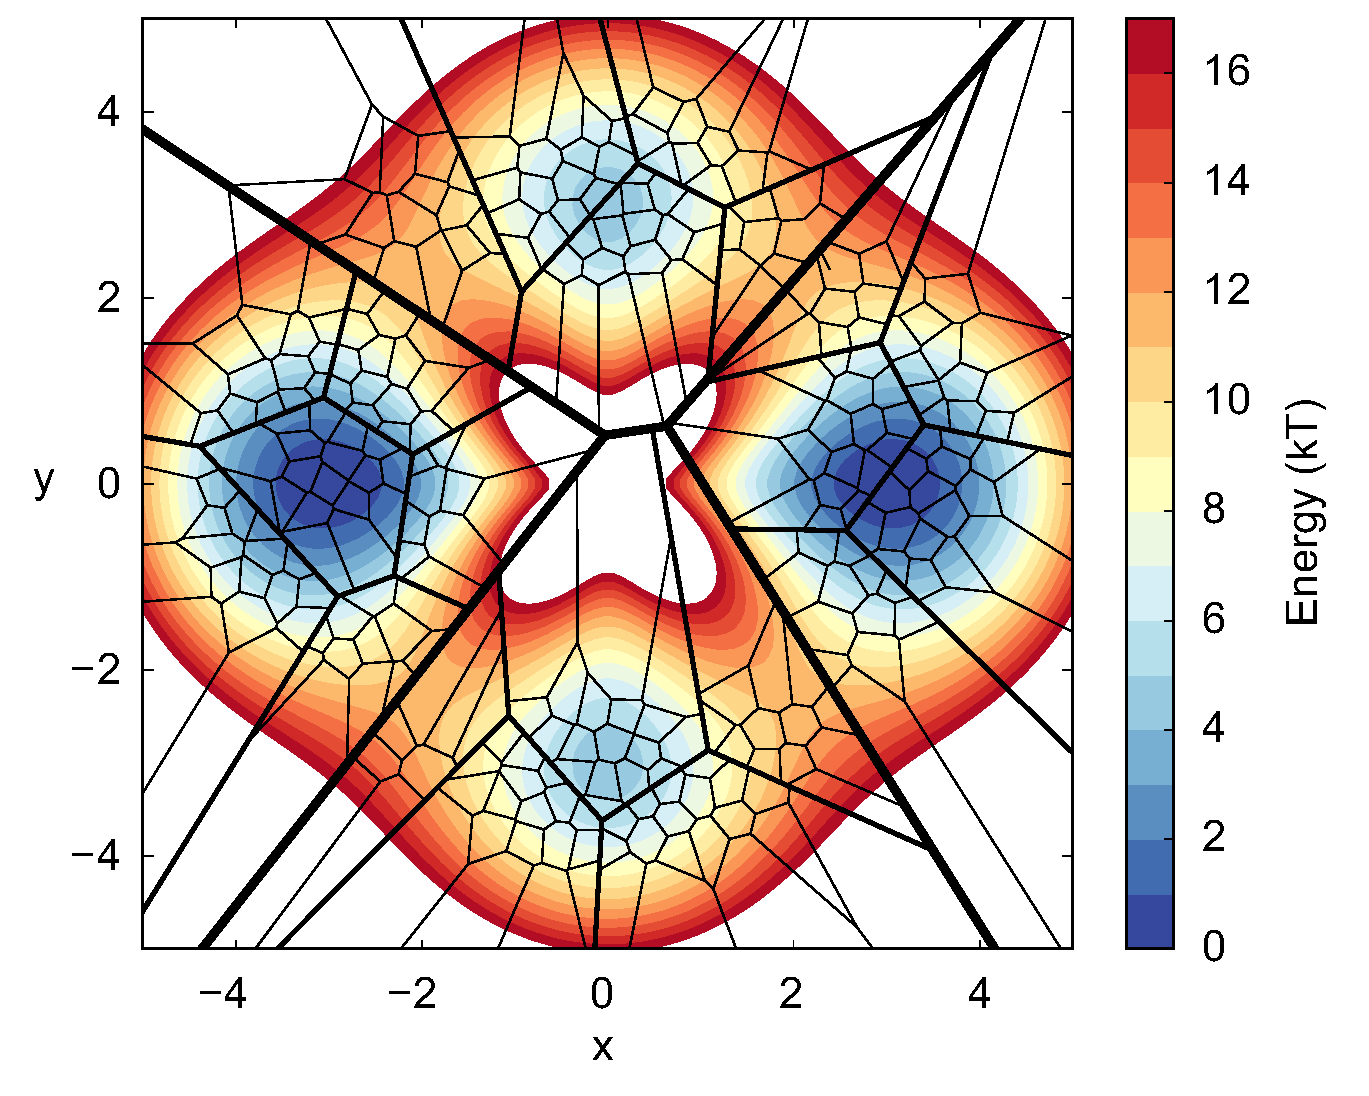
\includegraphics[width=\linewidth]{Figure2.eps}
\caption{Hierarchical Voronoi polyhedra for the Ring Potential model system \citep{Dickson2009,Adelman2013}.  
The blue colors show potential energy minima on the left and right and shallower minima on the top and bottom. 
Heavy lines show the Voronoi boundaries between the largest regions; one region is defined per local energy minimum.  
Each of these is broken up by medium regions (shown with medium-weight lines), which are themselves broken up by smaller regions (shown with light-weight lines).}
\label{fig:view}
\end{figure}
%%%%%%%%

\textbf{Choice of Distance Metric.} Similar to the choice of progress coordinate in conventional WE, the distance metric used in WExplore should capture the slow degrees of freedom that are relevant to the process of interest. 
The distance metric could for instance be an RMSD (root mean squared distance) measurement, but focusing only on a subset of the system atoms. 
For instance, a common distance metric used in ligand (un)binding simulations is calculated by aligning using binding site atoms, and calculating the RMSD between the ligands, without any further alignment \citep{Dickson2016}. 
Alternatively, a series of $N$ progress coordinates can be calculated as ${\bf X} = {\chi_1, \chi_2, \chi_3, …, \chi_N}$, and the Euclidean distance between two progress coordinate vectors can be used as the distance metric: $d_{ij} = |X_i - X_j|$. 
Many other examples are possible, and the researcher is only limited by their imagination. 
The distance used does not need to be differentiable or continuous.

\textbf{Region Size, Number of Levels, Branching Factor.} Once the distance metric is defined, the best practice is to run a short, straightforward simulation and observe the scale of fluctuations.
To be effective, the smallest region size (at the lowest level of the hierarchy) should be just outside the reach of the typical fluctuations observed in a time period $\tau$. 
This ensures that the first cloning events will correspond to significant differences between trajectories. 
At the other end, the largest regions should be big enough that a set of $B$ regions can evenly tile the space of interest, where $B$ is the branching factor. 
Typically, $B$ is set to 10, which is low enough to offer a big efficiency boost in region assignment, and high enough that branch factor overflows (where the simulation attempts to create a region higher than the branch number) do not occur early on in the simulation. 
The optimal number of levels between the smallest and the largest region sizes is system dependent. 
If simulations are routinely getting stuck on one level for long time periods, this could indicate that the spacing between levels is too large. 
If simulations very easily proceed from one to the next then the spacing might be too small. 
It is difficult to know beforehand what the optimal spacing will be, but suitable parameters can be easily found using a little common sense and a bit of trial-and-error.

\textbf{Number of Trajectories.} In contrast to conventional WE, WExplore does not employ a fixed number of trajectories (N\textsubscript{t}) per region. 
This would be wildly impractical, as the typical total number of regions is very large (e.g. 10,000 for a branching factor of 10 and a four-level hierarchy). 
Previous applications have aimed to choose N\textsubscript{t} to be as small as possible, while still allowing for simultaneous sampling of all states of interest, with a convenient value being 48, which is nicely congruent with 4-, 6- and 8-GPU compute servers \citep{Dickson2017,Dixon2018,Lotz2018}. 
A larger value will result in more consistent runs, while a smaller value allows for longer runs and more replicates. 
In practice we have found that single WExplore runs show high autocorrelation regardless of the value of N\textsubscript{t}, and that averaging over multiple replicates is a necessity, both to accurately compute observables and to estimate their uncertainty.

\section{Cluster-Specific Considerations}

To take full advantage of WESTPA’s scaling and parallelizability, users may seek to run the software on HPC clusters.
The tutorials included herein are written with the goal of teaching new and relatively inexperienced users the basics of using the software and therefore do not focus on optimizations pertaining to the code. 
We recommend that users become familiar with running WESTPA on a cluster, especially the cluster-specific issues and considerations that may arise.

\subsection{Minimizing the Number of Output Files}

It is advisable to minimize the number of output files generated by your simulation as this reduces the I/O overhead and will therefore be less taxing on the filesystem of the computing cluster. 
We recommend saving only the restart files that are necessary for continuing trajectories and analysis of the simulation. 
If the user needs additional information (e.g. coordinates that have been saved at a greater frequency than the $\tau$ value) contained in certain output files, those files should of course be kept. 
To further reduce the number of files, we suggest separately tarring up the files for each WE iteration. 
The resulting tarballs will also facilitate any transferring of your simulation data to another location. 

In some cases such as WE simulations that are run using GPUs, trajectory segments can complete too quickly, leading to a bottleneck where the transfer of files over the network to the local storage of the node is too slow or there are too many transfers over the network. 
In such cases, copy over the data of the entire previous WE iteration as a tarball  to the local storage of the node, run the entire iteration from this local storage, and copy back the results to the scratch space in a single tarball. 
While these transfers over the network will add some overhead to each WE iteration, they will avoid the network bottleneck. 

\subsection{Data Management}

A single WE simulation may generate multiple terabytes of data, presenting a challenge for storage and retrieval of data. 
Moreover, short trajectory segments in WE simulations commonly result in large numbers of small files, which are managed more slowly on some file systems than a smaller number of large files with the same overall disk size. 
To alleviate these potential issues, we recommend the following:

\begin{enumerate}
\item Perform an initial run to monitor data storage and retrieval. 
Note that the initial number of trajectory segments may be a small fraction of the amount that would be generated in the eventual production run. 
\item Delete unnecessary files as each trajectory segment is simulated (see example \verb|runseg.sh| files in the Basic and Intermediate Tutorials). 
Unnecessary files may include input files, log files from analysis tools, and raw text output files from analysis tools. 
Often, useful data from log files (e.g., temperature from an MD simulation) may be extracted from the log files and saved as auxiliary data to the WESTPA data file (\verb|west.h5| file), which stores data more efficiently than raw text.
\item Tar and optionally compress data from each WE iteration. 
This strikes a balance between excessive file count and excessive file size, either of which is typically sub-optimal for long term storage, especially on tape systems that may not guarantee the integrity of large files.
\item Consider saving coordinates for only the solute atoms of your system to an H5 file.
\end{enumerate}

\subsection{Minimizing Network Traffic Across Multiple Computing Nodes}
Given the large scale of a WESTPA simulation, it is advisable to limit the number and frequency of network operations (e.g. I/O operations and file transfers from the local disk to the global filesystem). 
We recommend the following strategies for reducing network traffic:

\begin{enumerate}
\item Perform a code scaling test to identify an appropriate $\tau$ value (see Section 3 above). 
\item Set environment variables to the full pathnames of repeatedly used programs (e.g. analysis tools used to calculate progress coordinates; see Basic Tutorial below).  
\item Copy repeatedly accessed files (e.g. reference structures and analysis scripts) to local scratch space and temporarily write the output files to this scratch space. 
After each trajectory segment of length $\tau$ completes, tar the output files, and copy the tarred files to the globally accessible filesystem using \verb|rsync|. 
\end{enumerate}

\subsection{Advice when Using GPUs}

If your WE simulation has extremely frequent starting up of simulation segments, your simulation may overheat gaming GPUs and potentially damage the hardware. 
For example, folding simulations of the NTL9 protein in implicit solvent with a $\tau$ value of 15 ps resulted in such issues on gaming GPUs (i.e. NVIDIA GTX 1080Ti GPUs) while the same simulations have no such issues on professional-graphics-programming GPUs. 
Coarse-grained simulations (residue-level models and coarse-grained) with high I/O are also problematic on gaming GPUs. 

\section{Uncertainty Quantification and Monitoring of Convergence}

Although they can report on much longer timescales, WE calculations still have limitations analogous to those of conventional MD simulations -- namely, force field inaccuracy and inadequate sampling. 
Assessing convergence requires care, as noted below. 
Even if sampling is adequate, as with any simulation result, error bars are required to set the results in context because there is always a finite range of results which are predicted in any stochastic calculation \citep{Grossfield2019}. 
Error analysis is particularly challenging because WE results ultimately depend on a large number of trajectories which typically are significantly correlated with one another due to repeated replication (“splitting”) events. 
Over the years, different error analyses have been employed \citep{Zhang2007,Zwier2016,Mostofian2019}. 
Here we give a brief overview of current practice.

The primary recommendation is to perform multiple, fully independent WE simulations when possible.
To understand the variation intrinsic to WE sampling, we suggest performing these runs from identical starting states. 
The data from these runs will not go to waste, as it can be combined for estimating observables, convergence, and error bars. 
When multiple runs are not feasible for a large-scale application, a sufficiently large number of trajectories/bin (at least 4 trajectories/bin) should be used to increase the chances of obtaining a diverse ensemble of pathways. 
To further enhance the diversity of the pathways, we recommend starting the simulation from multiple starting states when that is physically appropriate such as in protein binding. 
We note that a single run with a large number of trajectories/bin (4-50 trajectories/bin) has been shown to be more efficient in calculating rate constants than multiple runs with a small number of trajectories/bin (i.e. < 4 trajectories/bin) for molecular association/dissociation systems \citep{Pratt2019}. 

We focus here on understanding uncertainty in rate-constant estimation. 
First, there is the issue of “convergence”: how much time is required to obtain a result without systematic bias that is governed only by statistical noise? 
In a typical simulation started in a single state (A), the rate constant into a target state B is estimated by the steady-state probability flux into B -- i.e., the amount of probability arriving per unit time as sketched in Figure 3. 
However, there is a transient regime before the flux levels off to its steady value, and it is unknown in advance how long the transient will last. 
Of course, one should examine the time-dependence of the average flux (averaged over all WE runs) by eye, but this is unlikely to be sufficient. 
In addition, one can plot the flux as a function of some continuous coordinate which progresses from A to B: in steady state, the flux will be constant along any such coordinate \citep{Jeremy2019}.
Finally, we recommend using a “history augmented” Markov state model (haMSM) employing very fine bins/microstates, which can be built from the WE data as a different means for estimating steady-state flux values which can be compared to those measured directly in WE simulation \citep{Jeremy2019}. 
Alternatively, the impact of transient effects on rate-constant estimation can be reduced by incorporating the distribution of event durations (excluding dwell time in the initial stable state) that correspond to pathways captured by the simulation. 
This strategy has been shown to yield rate constants using a fraction of the simulation time required by the original WE method \citep{DeGrave2019}. 

Once the transient has completed, if multiple runs were performed, it is necessary to estimate the uncertainty in the rate constant based on the group of independent WE runs. 
The flux curves from the individual runs, plotted as a function of molecular time, may vary significantly as sketched in Figure 3. 
This large variation invalidates typical uncertainty estimation schemes based on the standard error of the mean, and we therefore recommend employing a Bayesian bootstrapping procedure \citep{MostofianJCTC2019}. 
This approach appears to be better than alternative approaches for handling estimates which vary over orders of magnitude, but we emphasize that the nominal 95\% “credibility regions” produced are overly optimistic and only cover the true mean a much smaller percent of the time \citep{MostofianJCTC2019}.

%%%Fig 3%%%
\begin{figure}
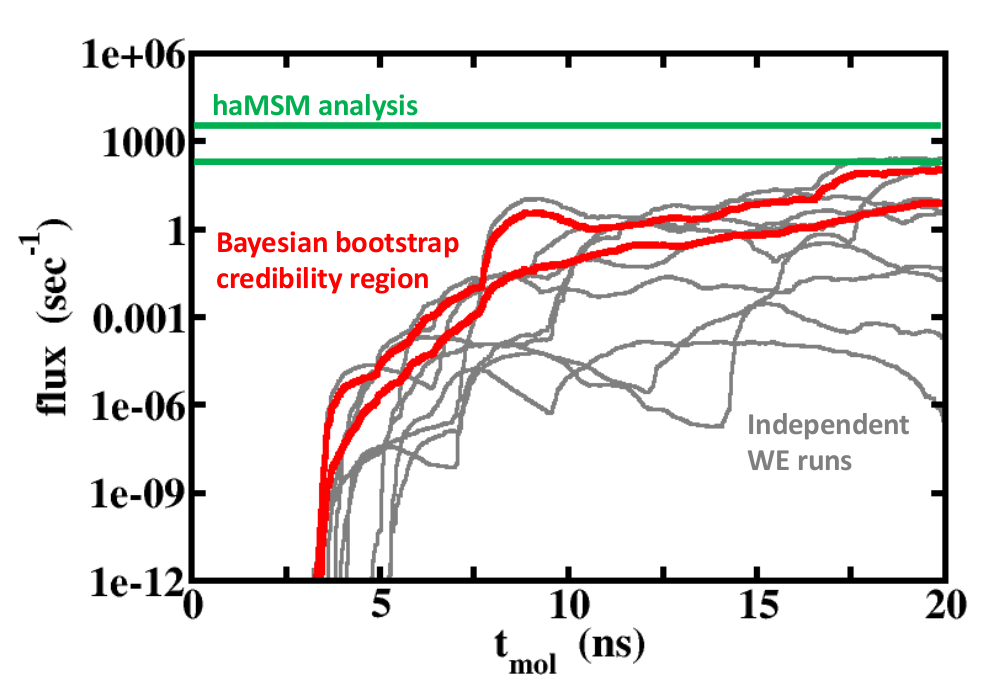
\includegraphics[width=\linewidth]{Figure3.png}
\caption{Convergence assessment and error analysis in the face of large run-to-run variation. 
The flux of probability into the target state B computed as a function of continuous molecular time, $t_{mol}$, is shown for several independent WE runs (grey). 
The large variation among individual runs makes it challenging both to assess whether the transient period has ended and to construct reliable error bars (see text). 
The history augmented Markov State Model (haMSM) analysis (green lines) provides an estimate of the long-time behavior, and the Bayesian bootstrap credibility region (red lines) estimates the average transient behavior.}
\label{fig:view}
\end{figure}
%%%%%%%%

\section{Tutorials}

\subsection{Basic Tutorial: Na\textsuperscript{+}/Cl\textsuperscript{-} Association}

\subsubsection{Introduction}

This tutorial involves carrying out a WE simulation of a molecular association process: Na\textsuperscript{+}/Cl\textsubscript{-} association. 
A user having completed this tutorial should be able to set up a simple WE simulation using the WESTPA software and develop an intuition for how changes in the WE parameters will influence the efficiency of sampling a process of interest, thus allowing that user to choose appropriate parameters for that process.

\textbf{Learning Objectives.} Though we strive to make the WESTPA software as user-friendly as possible, there are many system-specific parameters that must be carefully specified. 
The purpose of this basic tutorial is to introduce a new user to WESTPA and have that user become familiar with the flow of setting up and running a WE simulation.   

Specific learning objectives are:
\begin{enumerate}
\item Become familiar with the main simulation directory layout
\item Choose a progress coordinate
\item Choose an appropriate binning scheme
\item Prepare input files
\item Monitor a simulation
\end{enumerate}

\subsubsection{Prerequisites}

Users should install the latest version of the WESTPA software package, either by cloning from Git and compiling or through Conda. 
Installation instructions can be found on our website. 
Users will need to have Python 2.7 installed in order to use WESTPA. 
For analysis of simulation data, the \verb|hdfview| software greatly facilitates the visualization of large datasets. 
We will make use of that program in the ‘Analysis’ section of this tutorial.

Users should have basic knowledge of command line usage and the Python programming language. 
Since WESTPA is designed to conveniently interface with any external dynamics engine, users will also need to have experience using an MD engine (Amber, Gromacs, etc.). 
This tutorial will not provide instructions on how to use those engines; only how to interface the engines with WESTPA. 
In addition, a knowledge of analysis programs (such as Amber’s \verb|cpptraj| program or the MDAnalysis software is necessary and will not be covered here. 
This tutorial will go over examples of the various input files that are necessary for interfacing with WESTPA. 
This tutorial also assumes the user has some knowledge of the WE strategy, as its basic theory is not discussed herein.

\textbf{Computational Requirements.} A user should set aside at least 18 GB of disk space. 
This simulation took \textasciitilde 50 hrs to complete using 1 Intel Xenon 3.50 GHz CPU core.

This tutorial uses OpenMM version 7.3 for dynamics propagation (\url{http://openmm.org/}) and MDTraj 1.9.3 for progress coordinate calculations (\url{http://mdtraj.org/1.9.3/). System setup and equilibration was performed separately in OpenMM. A minimum version of 3.1.0 for HDFView is required for H5 file analysis.}

\subsubsection{Setting up a WE Simulation Using WESTPA}

\textbf{Overview.} WESTPA is run by calling the \verb|w_run| program from the command line with the appropriate options. 
This is normally done by running the \verb|run.sh| script from the main simulation directory. 
The simulation will then run until it has either completed the number of iterations specified by the user or has run out of time. 
Both of these parameters can be adjusted. 
Before a simulation can be run, however, the system must be initialized by calling the \verb|w_init| program from the command line with the appropriate options. 
This is normally done by running the \verb|init.sh| script from the main simulation directory.

Therefore, assuming the system is set up properly and all parameters have been properly specified, the WESTPA simulation can be run with the following at the command line (throughout our suite of tutorials, the command prompt is indicated with \$, which itself is not part of the commands that should be entered by the user):
 
\verb|$ ./init.sh|

\verb|$ ./run.sh|
 
Data from a WESTPA simulation will be stored in a file called \verb|west.h5|, which is an H5 file that can be opened with Python’s h5py package or with a graphical interface such as hdfview.

To monitor the simulation’s progress, we will use  the \verb|w_pdist| program of WESTPA. 
This will generate probability distributions (histograms) as a function of the progress coordinate and will enable the user to view those histograms with the plothist program. 

A WESTPA simulation, even after the requested number of iterations, may not be “complete.”  
Completion is assessed by whether some observable has converged to an expected or steady value. 
The choice of this observable is up to the user. 
To obtain these observables (such as the flux or rate constant), one will have to access the data in the H5 file and plot it using Python’s \verb|matplotlib| package (or another equivalent package).

Once a simulation is deemed complete, users can make use of the WESTPA analysis tools suite of programs, specifically \verb|w_ipa| in order to extract relevant data from the H5 file.

\textbf{The System.} To obtain a basic understanding of WESTPA’s parameters and learn how the software works, we will begin by studying the molecular association of Na\textsuperscript{+} and Cl\textsuperscript{-} ions. 
Our system will consist of a single Na\textsuperscript{+} cation along with a single Cl\textsuperscript{-} anion modeled with Joung and Cheatham parameters \citep{JoungCheatham2009} and solvated in a box of TIP3P water molecules \citep{tip3p}. 
These ions are initially dissociated at a separation distance of 12 \AA. 
The system was prepared using OpenMM and the appropriate input files are provided under “westpa\_tutorials” on GitHub, where you will also find a copy of this tutorial’s simulation directory (\verb|beginner_nacl|). 
We will not cover how the input files were generated or the rationale behind choices made when setting up the system (e.g. force field, water model etc.).


\textbf{Choosing an Initial State.} In looking at the association of two entities, especially thinking about how to extensively sample this process, there are some things we want to consider before we begin WE.
The first is how our initial state should look. If we choose to place the ions too close together, we may only observe one “type” of binding pathway, since the ions will not have as much time to orient themselves before binding. 
In reality, ions are symmetrical and we will not need this consideration but this would be an issue when determining how far apart to space, say, a drug and protein system or two protein binding partners. 
We also do not want to space the ions too far apart, as that would unnecessarily increase the time needed to observe binding events. 
We will therefore choose a generous distance of 12 \AA.

The coordinates (and velocities) of this starting structure, \verb|bstate.chk|, are placed in the \verb|bstates/| directory. 
This is an OpenMM checkpoint file, which I saved after equilibration.  
This is the file needed to directly resume dynamics.  
Depending on the dynamics engine you are using, this file will be different but will have the same function (for instance, an Amber restart file would be placed here if one were using \verb|sander| to run dynamics).
Also in this directory is a file named \verb|bstates.txt|. 
This file contains the name of our basis state structure and the probability of it being chosen if we want to sample a variety of initial structures (since we only are preparing one basis state, that probability is just 1). 
To more fully sample the configurational space of some process, it is often prudent to include more than one initial structure. 
In that case, all of those structure files can be placed in this directory with their names and probabilities included in the \verb|bstates.txt| file.

\textbf{Files for Dynamic Propagation.} Also necessary for running an Amber simulation are the topology and simulation input files. 
Those two files (\verb|bstate.pdb| and \verb|nacl_prod.py|) are placed in the \verb|common_files/| directory. 
This is a catch-all folder for any files needed while running dynamics. 
Notice that our $\tau$ value is defined in the \verb|nacl_prod.py| file, which is a Python script that runs OpenMM.  
This is the length of each WE iteration; so if the MD input script will run dynamics for, say, 10 ps then your $\tau$ value is 10 ps. 
This number needs to be carefully chosen depending on your system of interest. 
For this simulation, we will use a $\tau$ value of 50 ps. 

\textbf{Preparing the System Environment.} Next, we will want to make sure that WESTPA can properly access the MD engine we want to use and set up our simulation environment properly. 
These variables are all defined in the \verb|env.sh| file. 
You will need to open that in \verb|vim| or another text editor and make sure that your WESTPA environment is being sourced correctly (only if you are not using the Conda environment) and that your dynamics environment is being sourced correctly. 
It is also advised to set the runtime command variables for more efficient system calls if applicable.

\textbf{Equilibrium vs Steady State WE.} Now, let’s examine the \verb|init.sh file|, which initializes the simulation. 
In this file, we can specify whether to run an equilibrium or steady state simulation. 
The file in the tutorial directory is set up to run a steady state simulation. 
This is specified with the definition of the \verb|TSTATE_ARGS| variable and its use in the \verb|w_init| command. 
To run an equilibrium simulation, simply delete those two lines.

The choice of whether to run an equilibrium vs steady state simulation will depend on the research question being asked. 
Where do we want the system to go?  
Equilibrium simulations can be efficient in exploring configurational space, sampling ensembles of conformations. 
On the other hand, steady state simulations, where trajectories that reach some target state are recycled back to the initial state (along with their trajectory weights), can be more efficient in generating rate constants, and for exploring pathways towards some known target state. 

In our simulation, we do have a specific target state in mind and we know exactly what it looks like: Na\textsuperscript{+} and Cl\textsuperscript{-} interacting ionically at a close distance. 
We will therefore prepare to run a steady state simulation. 

\textbf{Progress Coordinate, Binning Scheme and $\tau$ value.}  For any WE simulation, we recommend choosing a progress coordinate that monitors the slowest relevant motion(s) such that faster motions will “go along for the ride.” 
The efficiency of generating pathways is tightly coupled to the choice of progress coordinate, along with how you choose to divide up that coordinate into bins. 
For the molecular association process involving the Na\textsuperscript{+} and Cl\textsuperscript{-} ions, a logical choice of progress coordinate would simply be the distance between the two ions, assuming that the surrounding solvent molecules respond relatively quickly to the positions of the ions. 
In other words, we can measure the simulation’s “progress” by how close the ions are to each other in a particular trajectory. 
This will turn out to be a good choice for our system, but for systems in which the binding partners involve ensembles of conformations, a pure distance-based progress coordinate will not be adequate and must be combined with a second dimension of the progress coordinate that tracks some other motion of the system.

Now that we have chosen a progress coordinate, we will need to consider our binning scheme. 
Imagine a space that contains all of the possible values of our progress coordinate. 
A good place to start is to perhaps define our progress coordinate as ranging from your initial state (basis state) to the initial definition of your target state and divide up this coordinate into 1-\AA{} wide bins. 
One way to obtain an initial definition of the target state for the Na\textsuperscript{+}/Cl\textsuperscript{-} association process is to subject a model of the associated Na\textsuperscript{+} and Cl\textsuperscript{-} ions to energy minimization using the same force field that will be used during the WE simulation and calculate the resulting distance between the ions using \verb|cpptraj|. 
This distance ended up being 2.6124 \AA{}, so we will set 2.60 \AA{} as our target state progress coordinate value. 
We recommend choosing the most strict definition possible for the target state for the recycling of trajectories in a steady state WE simulation to enable the use of more lenient definitions after the completion of the simulation. 
Make sure to add this number to \verb|tstate.file| in the main simulation directory, where your steady-state target state definition should always be placed.

Back to our bin definitions. 
If we choose to space our bins by ones from 2.6 to 12 \AA{} by 1’s (or some similar increment), this can lead to your simulation stalling. 
The bins may be too large with respect to your $\tau$ value and progress coordinate and trajectories cannot move to the next bin before a round of combination and replication occurs. 
It is a good idea, therefore, to run a short (10-20 iterations) WESTPA equilibrium simulation to see how your trajectories are progressing with the WE parameters you have set.
If necessary, adjust the binning or include an additional dimension to your progress coordinate.

Here is the preliminary binning scheme we will employ, which is defined in the \verb|west.cfg| file:
 
\verb|[0.00, 2.60, 2.80, 3.00, 3.20, 3.40, 3.60, 3.80,|

\verb|4.00, 4.50, 5.00, 5.50, 6.0, 7.0, 8.0, 9.0,|

\verb|10.0, 11.0, 12.0, 13.0, 14.0, 15.0, ‘inf’]|
        	 
Notice how we start at 15 \AA{} (a little bit beyond our initial value of 12 \AA) and increment by ones, but as we get closer to our initial state of 2.60 \AA, we start incrementing more finely. 
This finer binning will help to collect probability closer to our target state and promote more binding events.

\textbf{Other WE Parameters.} The following WE parameters are discussed along with where they are specified in the parameter files. 
First, make sure you have chosen an  appropriate $\tau$ value (see Section 3) and that it is properly specified in your dynamics input file. 
As mentioned above, the $\tau$ value, along with the number of trajectories per bin, is coupled to the choice of progress coordinate and binning scheme. 
We recommend starting with \textasciitilde 4-5 trajectories/bin. 
This value is specified in the \verb|west.cfg| file as \verb|bin_target_counts|. 
Make sure that the frequency at which conformations are saved in your trajectories (as indicated in your dynamics input file, e.g. \verb|md.in| for Amber) matches the number of elements in the pcoord array of the \verb|west.cfg| file. 
We recommend running the simulation for a short time to test the effectiveness of the WE parameters, setting \verb|max_total_iterations| to 10 in the \verb|west.cfg| file before letting the simulation run to a full 100 iterations.  

\textbf{Trajectory Imaging.} Since the replication and combination of trajectories in a WE simulation depends on the values of the progress coordinate, trajectories that are carried out with periodic boundary conditions should be imaged before calculating the progress coordinate (e.g., after completing each trajectory segment of length $\tau$). 
Otherwise, erroneous values of the progress coordinate may result from parts of the simulation system drifting outside of the periodic box. 
MDTraj, which is used to calculate the distance in this tutorial, is able to only calculate distances for nearest-image ion pairs (essentially what Amber does with the \verb|autoimage| command in AmberTools’ \verb|cpptraj| program.

\subsubsection{Initializing the WE Simulation}

To initialize the simulation, run the \verb|init.sh| script as mentioned before. 
You will see a body of text output indicating that the initialization has completed successfully. 
We will briefly present the key features of this script. 

As mentioned before, \verb|init.sh| calls the \verb|w_init| program, which in turn, runs a script in the \verb|westpa_scripts/| directory called \verb|get_pcoord.sh|. 
This script, in this tutorial, is very simple. 
It prints the contents of a file, \verb|pcoord.init|, and gives that to \verb|WEST_PCOORD_RETURN|.
The \verb|pcoord.init| file contains the progress coordinate value of the basis state, and so this operation essentially tells WESTPA which bin your basis state falls into. 
The \verb|pcoord.init| file is generated by running the \verb|get_distance.py| script in \verb|common_files/| on \verb|bstate.chk| and redirecting the output into a file named \verb|pcoord.init|. 
Initializing your system this way is often a good idea, as it allows you to test out your particular method of progress coordinate calculation.  
However, \verb|get_pcoord.sh| can calculate the progress coordinate directly (see Intermediate Tutorial), or run whatever script you need to do so.  
In fact, \verb|get_pcoord.sh| can include any additional commands; this built-in flexibility allows you to perform operations on your basis states before beginning the WESTPA simulation. 

\subsubsection{Running the WE Simulation}

To carry out the simulation, run the \verb|run.sh| script as mentioned before. 
You will not see any output. What \verb|run.sh| does is call \verb|w_run| which, among other things, runs the \verb|runseg.sh| script that is in the \verb|westpa_scripts/| directory. 
This script will run dynamics each iteration, calculate a progress-coordinate value for the updated structure and then return that value to \verb|WEST_PCOORD_RETURN|. 

In this tutorial, OpenMM is used to run dynamics (by running the \verb|nacl_prod.py| script) and MDTraj is used to calculate the progress coordinate (by running the \verb|get_distance.py| script).  
If a user wishes to change either the dynamics or analysis programs, these are the two locations where it will need to be done. 

For an example script for using Slurm to run a job on a computing cluster, see \verb|runwe.slurm|. 
You can adapt this template script to run WESTPA on your desired cluster.  

\subsubsection{Monitoring the WE Simulation}

We recommend checking the progress of your WE simulation every 10 iterations or so. 
This can be done with the \verb|w_pdist| program. To use this program, first stop the simulation (it can be started easily from the point it left off by running \verb|run.sh| again) and then call \verb|w_pdist|:
 
\verb|$ w_pdist|
 
This will produce a new H5 file called \verb|pdist.h5|. 
To see how our progress coordinate is evolving over time, we can use the plothist program with the evolution option:
 
\verb|$ plothist evolution pdist.h5|

This will produce a pdf file called \verb|hist.pdf|. 
Open this file, the contents of which are displayed in Figure 4. 

%%%Fig 4%%%
\begin{figure}
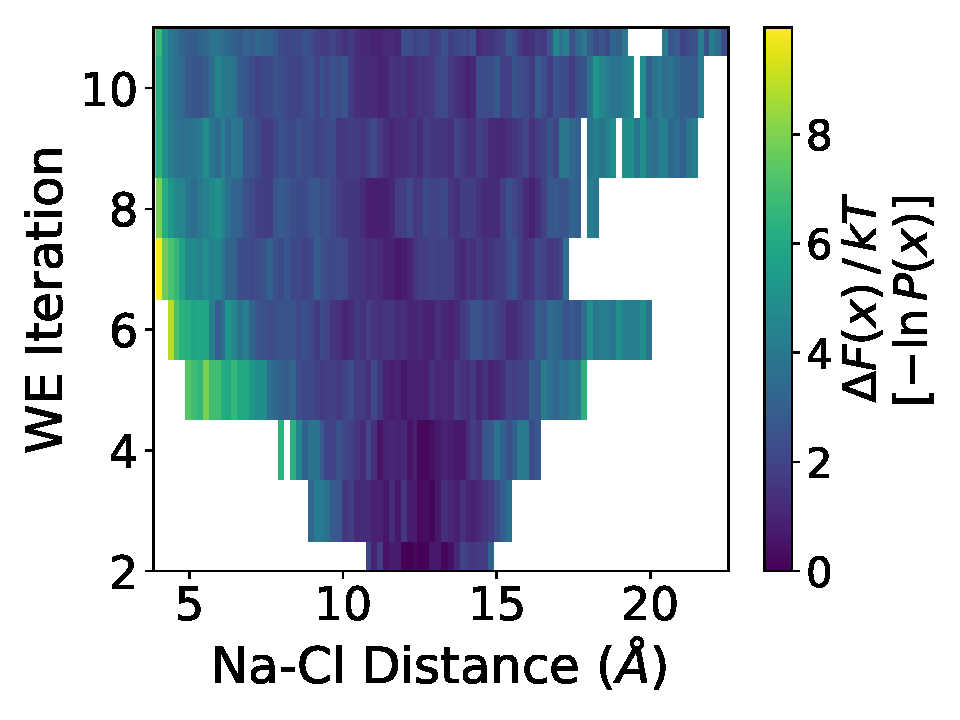
\includegraphics[width=\linewidth]{Figure4.pdf}
\caption{Probabiity evolution of Na\textsuperscript{+}/Cl\textsuperscript{-} association as a function of interatomic distance and WE iteration. 
The default output from plothist displays the histograms as the negative log of the probability. 
This can be adjusted by adding the appropriate command line options to plothist (run plothist -h for more information). 
The distribution from your particular simulation may look slightly differnet. 
Oberve that at the beginning of the simulation, the probability is centered around 12 \AA{} (our initial distance).}
\label{fig:view}
\end{figure}
%%%%%%%%

As expected, most of the probability at the start of our simulation is concentrated around the progress coordinate value for our initial state (10 \AA). 
As our simulation progresses, the probabilities fan out in both directions, with most of the probabilities moving towards larger values and some of the probabilities nearing our target value of 2.6 \AA. 
To see if your simulation has generated some successful binding events after only 10 iterations, run the following:

\verb|$ w_succ|
 
The example simulation had its first successful event after 14 iterations. 
The output will show (if a successful event occured) the iteration and segment number in which the first event occurred (e.g. iteration 14, segment 2).

You can trace this successful trajectory back to the basis state to obtain a complete trajectory with the \verb|w_trace| command. 
You will need to provide the iteration and segment of the successful trajectory as options separated by a colon:
 
\verb|$ w_trace 14:2|
 
The output will be written to the file \verb|traj_14_2_trace.txt|. 
That file contains the parents of the successful trajectory all the way back to the basis state. 

\verb|$ w_trace 14:2|
 
The output will be written to the file \verb|traj_14_2_trace.txt|. 
That file contains the parents of the successful trajectory all the way back to the basis state.

\subsubsection{Analyzing the WE Simulation}

One way to assess the convergence of our simulation is to determine when the primary observable of interest (i.e. the flux into the target state) levels off. 
To monitor the flux, we will first need to prepare our \verb|west.cfg| file to analyze the simulation. 
This is normally done be adding an analysis module to the end, which is already present in this tutorial’s files. 
Use this as a template for future analyses.

You will see that we create an analysis instance called \verb|TEST| and then define bins and states for this scheme. 
These bins are strictly for analysis and have nothing to do with our progress coordinate bins defined earlier. 
Since we only need to designate the bound and unbound states here, we define three bins:
 
\verb|[0.0, 2.6, 10.0, ‘inf’]|
 
The way that state definitions work is that you provide a coordinate in the configurational space and whichever analysis bin that coordinate is in becomes that state. 
For instance, our bound state definition is given by \verb|[0]|, so whichever bin above that the value 0 falls into will be our “bound” state. 
This is the bin from 0 to 2.6. 
The same goes for the unbound state (10.0 to infinity). 
The intermediate state does not need to be defined.

With these states defined we can now analyze how much probability, in the form of trajectories, is entering or leaving each state using the \verb|w_ipa| program, which will run two separate WESTPA tools, \verb|w_assign| and \verb|w_direct|. 
To generate the H5 files needed to analyze the fluxes, run the following from the main simulation directory:
 
\verb|$ w_ipa -ao|

You will see that a new directory titled \verb|ANALYSIS| has been created, inside of which is a subdirectory corresponding to our \verb|TEST| analysis scheme that was defined in the \verb|west.cfg| file. 
Inside of this subdirectory are our \verb|assign.h5| and \verb|direct.h5| files. 
The \verb|direct.h5| file is where the fluxes are stored. 
We can open it up with \verb|hdfview| and view all of the datasets.
 
The \verb|target_flux_evolution| dataset gives the flux over time (number of WE iterations) into each state we defined earlier. 
To view this dataset, double click on it. 
The 0th column corresponds to the flux into state 0, which we defined as our target state. 
The iter stop is at the beginning of that iteration, so if you had a binding event by iteration 10, observe the  flux into our target state. 
Highlight the “expected” column and click the plotting button in the upper-left hand corner to view the flux evolution as a function of 0-indexed iteration.
 
By iteration 10, the flux has most likely not levelled off, so our simulation cannot be considered converged. 
Let’s continue the simulation for a total of 100 WE iterations and analyze the resulting dataset. 
A completed H5 file is included in the \verb|for_analysis/| directory for your convenience.
Your plot should look something similar to Figure 5, which was generated in \verb|matplotlib|. 

%%%Fig 5%%%
\begin{figure}
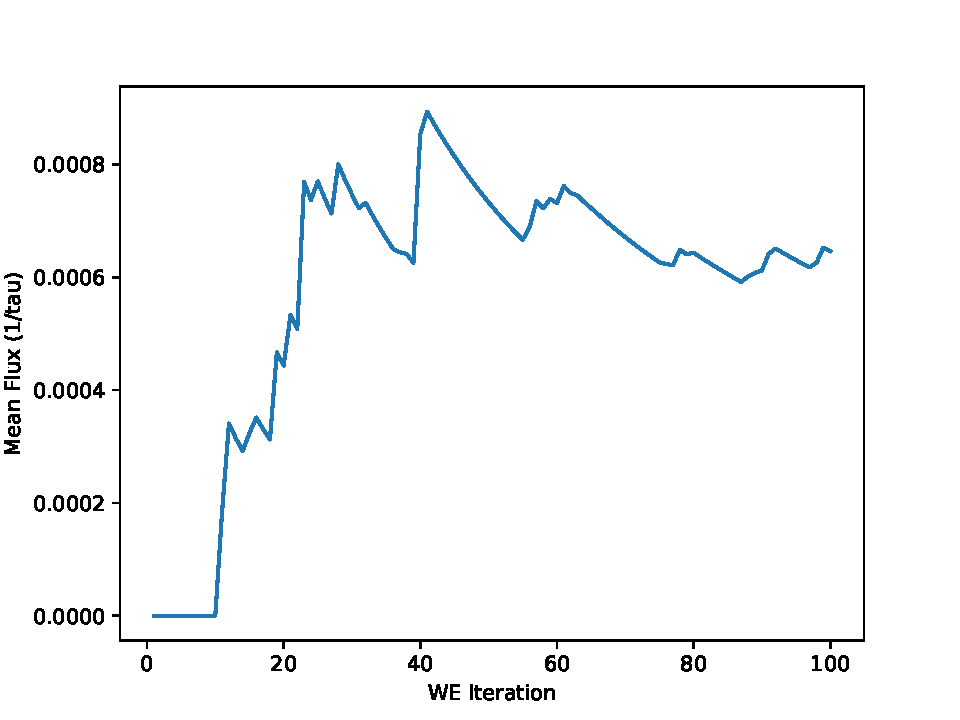
\includegraphics[width=\linewidth]{Figure5.pdf}
\caption{Mean flux evolution of Na\textsuperscript{+}/Cl\textsuperscript{-} association as a function of WE iteration. 
The mean flux alternatively rises sharply and then relaxes. 
These "peaks" correspond to probability crossing into the target state. 
Your plot may still not be completely converged after 100 iterations.}
\label{fig:view}
\end{figure}
%%%%%%%%

While the flux into the target state has not completely levelled off, it is much more steady than previously, so we can stop the simulation here and consider how much longer we should extend the simulation. 
For other systems, you may want to run the simulation longer for better convergence. 
You may also want to have additional criteria for convergence.

To visualize a trajectory, one must first identify a continuous series of trajectory segments in each iteration from the basis state to the target state. 
This will be given in the \verb|w_succ| output along with \verb|w_trace|, as we have done previously. 
However, you will also need to retrieve the trajectory file from each of those segments and combine them using \verb|cpptraj|. 
To automate this process, we have provided the \verb|amberTraj.sh| script, which can be adapted for other systems. 
This script uses the \verb|cpptraj| program available in AmberTools to extract the binding trajectory of a successful event.
The resulting trajectory file can be loaded along with the system topology into the VMD visualization software to generate a movie of the association process.
 
\subsubsection{Conclusion}

Hopefully at this point, you should have gained a good idea of the work flow required to set up, run, and analyze a WESTPA simulation using a simple progress coordinate. 
If you desire more complex options for your simulations (e.g. multi-dimensional progress coordinates) and further discussion of how to choose various simulation parameters, we highly suggest going through the other tutorials to get a sense of how that can be done.

\subsection{Intermediate Tutorial: P53 Peptide Conformational Sampling}

\subsubsection{Introduction}

Since the WE algorithm aims to fill empty bins in configurational space, WE simulations can be effective in the enhancement of conformational sampling \citep{Dickson2014,Zwier2015} as well as the generation of pathways and rate constants for rare events. 
This tutorial will focus on the conformational sampling of a peptide and instruct users on how to set up and analyze a simulation involving a two-dimensional progress coordinate. 
In addition, we will go over how the binning scheme can be chosen and adjusted accordingly to balance efficiency and performance.

\textbf{Learning Objectives.} This tutorial will help users develop a sense for which progress coordinates may be effective for conformational sampling of a peptide and how to bin along those progress coordinates.  

Specific learning objectives include:
\begin{enumerate}
\item How to set up a two-dimensional progress coordinate
\item How to monitor this coordinate as the simulation progresses
\item How to evaluate whether the binning scheme is effective
\item Combining and creating bins “on-the-fly”
\item Storing and accessing auxiliary data
\end{enumerate}

\subsubsection{Prerequisites}

Users should have completed the Basic Tutorial and have a potential progress coordinate in mind for their system of interest. 

\textbf{Computational Requirements.} This simulation required at least 10 GB of disk space and \textasciitilde 36 hours to complete (40 iterations) on a 12-core, 2.6 GHz Intel Xeon node.
This tutorial uses AmberTools19’s \verb|sander| package for dynamics propagation and the  \verb|cpptraj| package for progress coordinate calculations (\url{http://ambermd.org/AmberTools.php}).  
AmberTools is available free of charge.

\subsubsection{Adding Another Dimension to the Progress Coordinate}

While a one-dimensional progress coordinate can be effective for molecular association processes (e.g. Na\textsuperscript{+}/Cl\textsuperscript{-} in the Basic Tutorial), a two-dimensional coordinate may be necessary for more complex processes such as peptide/protein conformational transitions. 
To include another dimension to the progress coordinate, we first specify the progress coordinate dimensionality as “2” in the \verb|west.cfg| file. 
Next, we calculate the values corresponding to each dimension of the progress coordinate and pass the resulting two values at the same time to \verb|WEST_PCOORD_RETURN| in both the \verb|get_pcoord.sh| and \verb|runseg.sh| scripts. 
For example, if the first dimension of the progress coordinate has a value of 1 and the second dimension has a value of 5, (1 5) must be passed at the same time to \verb|WEST_PCOORD_RETURN| instead of sequentially as 1 and then 5. 
This can be done with the \verb|paste| command in bash (see example \verb|get_pcoord| and \verb|runseg| files). 
In addition, the bins will need to be given two lists for each of the two dimensions by adding dashed entries (one underneath the other) in the \verb|west.cfg| section for bin definitions. 
A user may also choose to define a two-dimensional binning scheme in a \verb|system.py| file.

\subsubsection{Preparing the WE System}

\textbf{The System.} We will focus on  the conformational sampling of a 15-residue, N-terminal peptide fragment of tumor suppressor p53 that has been thought to be disordered in its unbound state and adopts an $\alpha$-helical conformation upon binding the MDM2 protein. 
Simulations were run at 275 K using the Amber ff14SBonlysc force field \citep{ff} and generalized Born implicit solvent \citep{implicit_solvent}. 
As in the Basic Tutorial, we will not go into detail about how the files were generated in Amber or the decisions made in setting up the system with Amber.

\textbf{Choosing an Initial State.} Our WE simulation will be started from the MDM2-bound conformation of the p53 peptide. 
In particular, coordinates for the peptide conformation will be extracted from the crystal structure of the MDM2-p53 peptide complex \citep{Kussie1996}. 
This $\alpha$-helical conformation of the peptide will then be energy-minimized and equilibrated before subjecting the resulting, solvated system to a WE simulation.

\textbf{Files for Dynamics.} The topology file (\verb|P53.MDM2.prmtop|) and dynamics input file (\verb|md.in|) can be found in the \verb|common_files/| directory. 
In the \verb|md.in| file, it should be specified that the trajectory segment will be run for a length that corresponds to a $\tau$ value of 50 ps.

\textbf{Preparing the Simulation Environment.} See this subsection in the Basic Tutorial.

\textbf{Equilibrium vs Steady State WE.} In the \verb|init.sh| file, observe that all lines mentioning \verb|TSTATE_ARGS| have been removed. 
This signals WESTPA to run an equilibrium WE simulation in which we do not have a set target state. 
This is a good option when the goal of your process is to generate as many configurations as possible and you have no set target state in mind.

\textbf{Progress Coordinate, Binning Scheme and $\tau$ Value.} To extensively sample the conformations of the peptide, we might define a progress coordinate that monitors the extent of “unfoldedness” in the peptide using the RMSD of a given conformation from the initial structure. 
However, RMSD cannot differentiate among conformations that have the same large RMSD values. 
To further differentiate between such conformations, we can include another orthogonal measure of unfoldedness such as the end-to-end distance of the peptide. 

To determine a suitable binning scheme, we will start with an upper limit of 10 \AA{} for the heavy-atom RMSD dimension of the progress coordinate. 
Spacing the bins along this dimension by 1’s may be too large for any transitions to occur between bins so we opt for a finer bin spacing:

\verb|[0.0, 0.2, 0.4, 0.6, 0.8, 1.0, 1.4, 1.8,|

\verb| 2.2, 2.6, 3.0, 3.5, 4.0, 5.0, 6.0, 7.0,|

\verb| 8.0, 9.0, 10.0, ‘inf’]|

We will see how the trajectories progress and adjust accordingly. 
Notice that a bin spacing of 0.2 is not maintained for the entire length, as 50 bins even along one dimension would result in a very large number of total trajectories (4 trajectories per bin would result a total of 200 trajectories if all of the bins are occupied). 
Furthermore, care must be exercised in the addition of bins along a second dimension as the total number of trajectories can “blow up” to an enormous number of trajectory segments (e.g. 10,000).

To get a feel for how the end-to-end distance evolves in the simulation, let’s expand out from the initial distance of 28.5 \AA{} with 0.5-\AA{} wide bins in either direction:

\verb|[0, 20, 20.5, 21, 21.5, 22, 22.5, 23, 23.5,|

\verb| 24, 24.5, 25, 25.5, 26, 26.5, 27, 27.5, 28,|

\verb| 28.5, 29, 29.5, 30, 30.5, 31, 31.5, 32, 32.5,|

\verb| 33, 33.5, 34, 34.5, 35, 35.5, 36, ‘inf’]|

Our $\tau$ value should allow for successful transitions between bins of this spacing.

\textbf{Other WE Parameters.} Let’s run our WE simulation with 4 trajectories/bin for 40 iterations. 
Since the goal here is the conformational sampling of a peptide and we are running an equilibrium WE simulation, we do not need to define a target state.

\subsubsection{Tracking the Auxiliary Data}

While it is possible to go back after a simulation has run and calculate some value you wished you had kept track of, it can be tricky to do so (though possible with a tool called \verb|w_crawl| which is not discussed in this guide). 
We strongly recommend conducting all relevant analysis during the simulation and storing the resulting data as auxdata in the H5 file. 
In our case, we will  calculate and store the $\phi$/$\psi$ backbone dihedral angles of the peptide as auxdata for each of the sampled conformations.  

To signal for WESTPA to collect auxdata, you will need to add an auxiliary dataset into the \verb|west.cfg| file and make sure it is enabled. 
See the \verb|west.cfg| file in the tutorial directory for how this might look. 
You can name the dataset whatever you would like. 

Once you have specified the datasets and named them, you will need to add in commands to \verb|runseg.sh| that calculate those values and pass them to WESTPA system variables. 
The variables will be named \verb|WEST_XYZ_RETURN| where “xyz” was the name given to the dataset in the \verb|west.cfg| file initially. 
This can be treated analogously to the pcoord value and \verb|WEST_PCORD_RETURN|.

\subsubsection{Initializing and Running the WE Simulation}

Make sure that your \verb|get_pcoord.sh| and \verb|runseg.sh| files are calculating the RMSD and end-to-end distance and returning these values to \verb|WEST_PCOORD_RETURN|. 
The \verb|get_pcoord.sh| will calculate the initial progress coordinates using AmberTools’ \verb|cpptraj| program from within the script, as opposed to reading the value from an external file as in the beginner tutorial.
The \verb|runseg.sh| uses AmberTools’ \verb|sander| program for dynamics propagation and does so within the script.

\subsubsection{Monitoring the WE Simulation (10 Iterations)}

Once the simulation has run for about 10-20 iterations, copy the H5 file and run \verb|w_pdist| with the copied file. 
You can then use \verb|plothist| to view each dimension of the progress coordinates separately as the values evolve over the course of those few iterations:

\verb|$ plothist evolution pdist.h5 0 -o hist_dim0.pdf|

\verb|$ plothist evolution pdist.h5 1 -o hist_dim1.pdf|

Where the “0” or “1” after the \verb|plothist| command is the progress coordinate dimension (zero indexed). 
Observe the two probability distributions in Figure 6.

%%%Fig 6%%%
\begin{figure}
\centering
\begin{subfigure}[A]{0.35\textwidth}
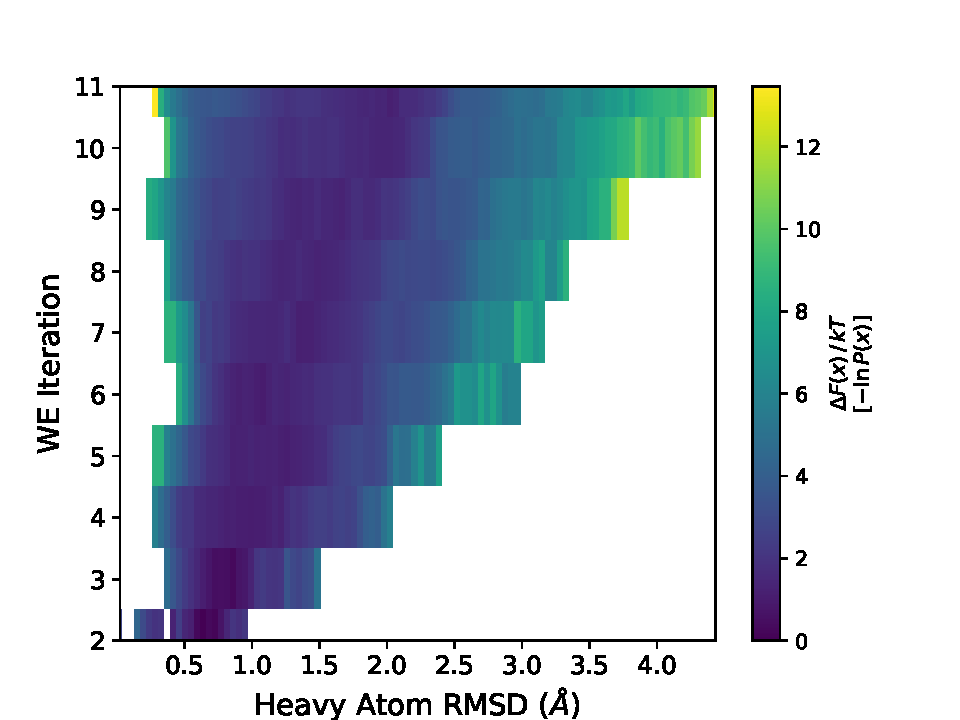
\includegraphics[width=\linewidth]{Figure6A.pdf}
\end{subfigure}
\begin{subfigure}[B]{0.35\textwidth}
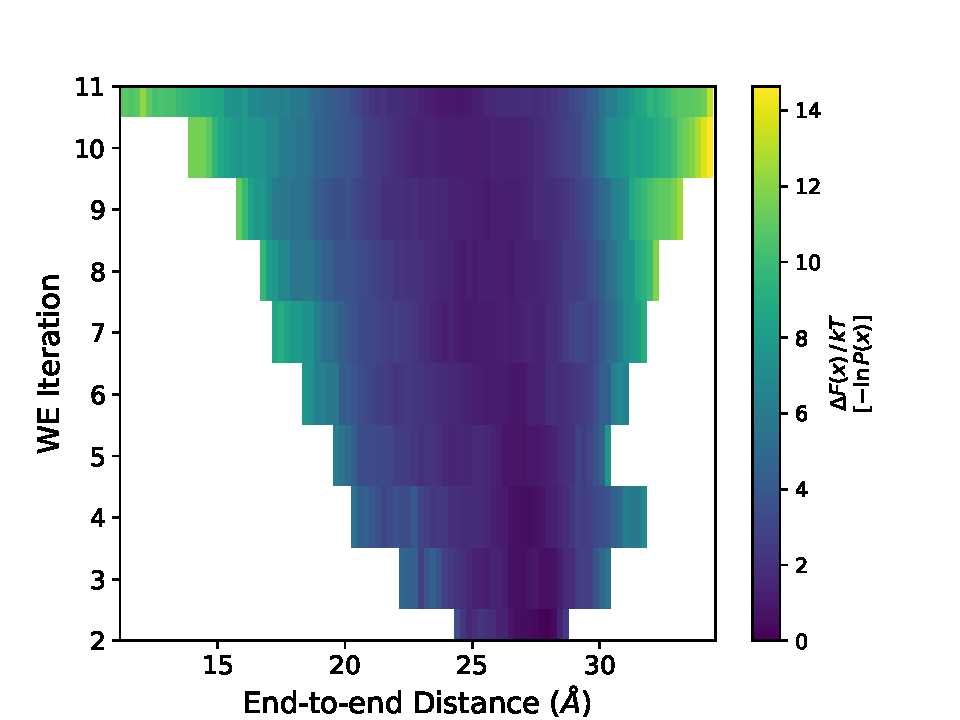
\includegraphics[width=\linewidth]{Figure6B.pdf}
\end{subfigure}
\caption{Probability distributions from plothist for each of the two progress coordinate dimensions versus WE iteration. 
The simulation was analyzed after 10 WE iterations.}
\label{fig:view}
\end{figure}
%%%%%%%%

\subsubsection{Adjusting Bin Spacings "On the Fly"}

The RMSD has reached a value of 4-5 \AA{} and the end-to-end distance has reached \textasciitilde 10 \AA{}, which is encouraging progress for only 10 iterations. 
Note that most of the probability (and therefore most of the computation) is still stalled in the initial states of 1-2 RMSD and 20-25 end-to-end distance. 
We can help  focus the computing power on the more interesting “edge” conformations by modifying the binning scheme before continuing the simulation.
  
In WESTPA, the binning scheme can be updated at any time since the trajectory weights are independent of the bins (and progress coordinate). 
To do so, first stop the simulation and then adjust the bins in your \verb|west.cfg| file. 
Re-start your simulation by running the \verb|run.sh| script again and the simulation will continue from where it left off. 
At the start of the next iteration, the new bins will have been implemented.  

In our case, I would like to focus sampling on higher RMSD values (3-4 \AA) instead of those \textasciitilde 1-2 \AA. 
To do this, I will collapse the bins from 0 to 1.8 and define some more bins past 10:

\verb|[0.0, 1.8, 2.2, 2.6, 3.0, 3.5, 4.0, 5.0, 6.0,|

\verb| 7.0, 8.0, 9.0, 10.0, 11, 12, 14, 16, 18, 20, ‘inf’]|

For the end-to-end distance, I will add more bins for the lower distances and collapse bins over 26. 
We would normally want to keep these bins over 26 but having fewer will shorten the runtime of this tutorial.

\verb|[0, 2, 4, 6, 8, 10, 12, 14, 16, 18, 20, 21,|

\verb| 22, 23, 24, 25, 26, ‘inf’]|

The reason we eliminated the initial 0.5 spacings is that this degree of freedom is readily explored in the system.

\subsubsection{Monitoring the WE Simulation (40 Iterations)}

After running the simulation for another 30 iterations (for a total of 40), we obtained the following updated probability distributions displayed in Figure 7.
The completed H5 file is included in \verb|for_analysis/| for your convenience.

 %%%Fig 7%%%
\begin{figure}
\centering
\begin{subfigure}[A]{0.35\textwidth}
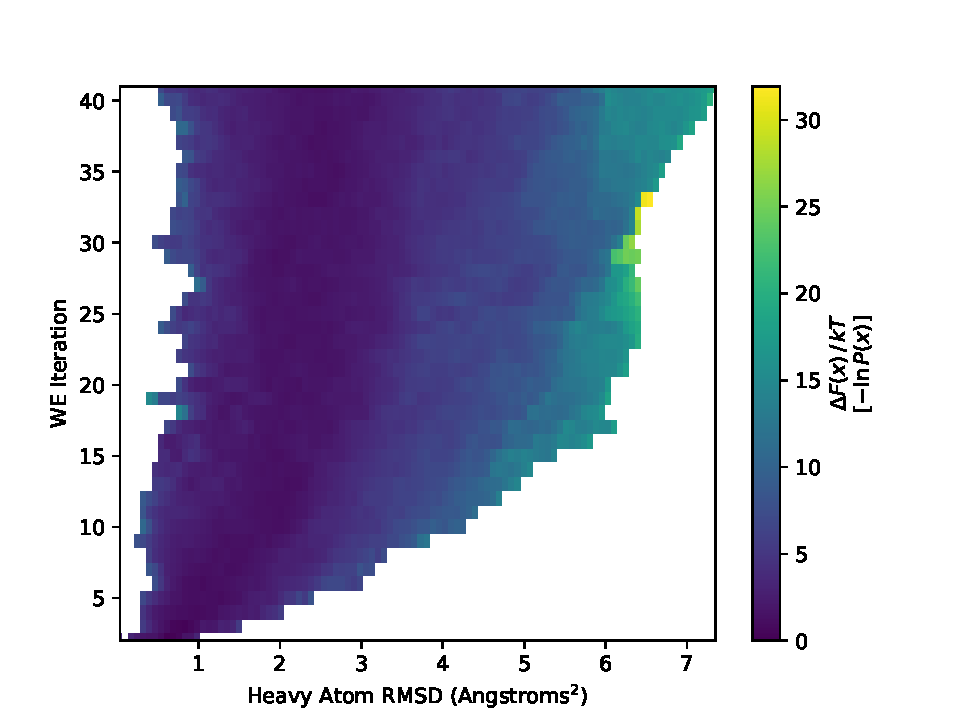
\includegraphics[width=\linewidth]{Figure7A.pdf}
\end{subfigure}
\begin{subfigure}[B]{0.35\textwidth}
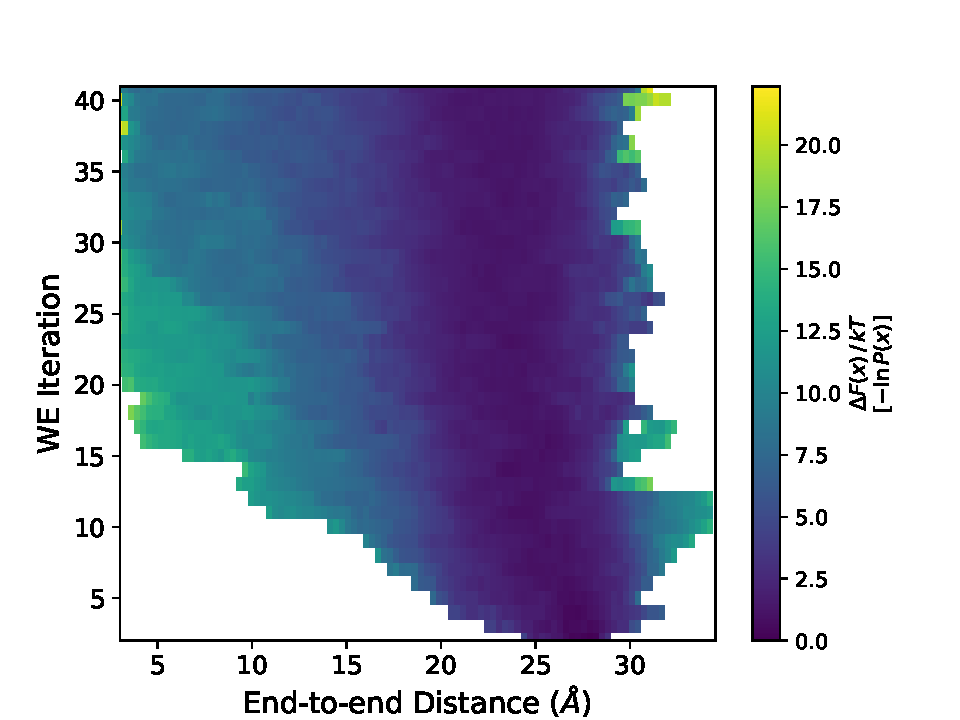
\includegraphics[width=\linewidth]{Figure7B.pdf}
\end{subfigure}
\caption{Probability distributions from plothist for each of the two progress coordinate dimensions versus WE iteration. 
The simulation was re-analyzed after 40 total WE iterations}
\label{fig:view}
\end{figure}
%%%%%%%%

The effects of the bin-modifications can clearly be seen in the case of the end-to-end distribution. 
No more trajectories with an end-to-end distance >30 can be seen after iteration 10, a result of the choice not to bin over 26 in that dimension.

The end-to-end distance seems to have reached 2-3 \AA{} around iteration 20. 
The RMSD plateaued a bit from iterations 20-30 but then proceeded to values around 7 \AA.  

Two lessons can be learned from these observations. 
First, if you do not have bins in a particular direction, you may not see sampling in that direction. 
Second, even though the RMSD coordinate appeared to have stalled around iteration 20-30, it eventually was able to surmount whatever barrier existed and attain some higher RMSD values. 
Patience is key, as a single trajectory may replicate to become many trajectories if it crosses into a new bin.

\subsubsection{Accessing Auxiliary Data}

To access the auxdata from the H5 file, you can open \verb|west.h5| in \verb|hdfview| but this will not allow you really use the data. 
To plot all of the dihedrals as a Ramachandran plot in \verb|matplotlib| as I have done in Figure 8 (actually, we just did so for the second dihedral, but you could extend it to all if you so desire), you will need to utilize the \verb|h5py| package in Python to extract the values you need from the H5 file and then plot them. 
The plotting script is included in the tutorial directory.

%%%Fig 8%%%
\begin{figure}
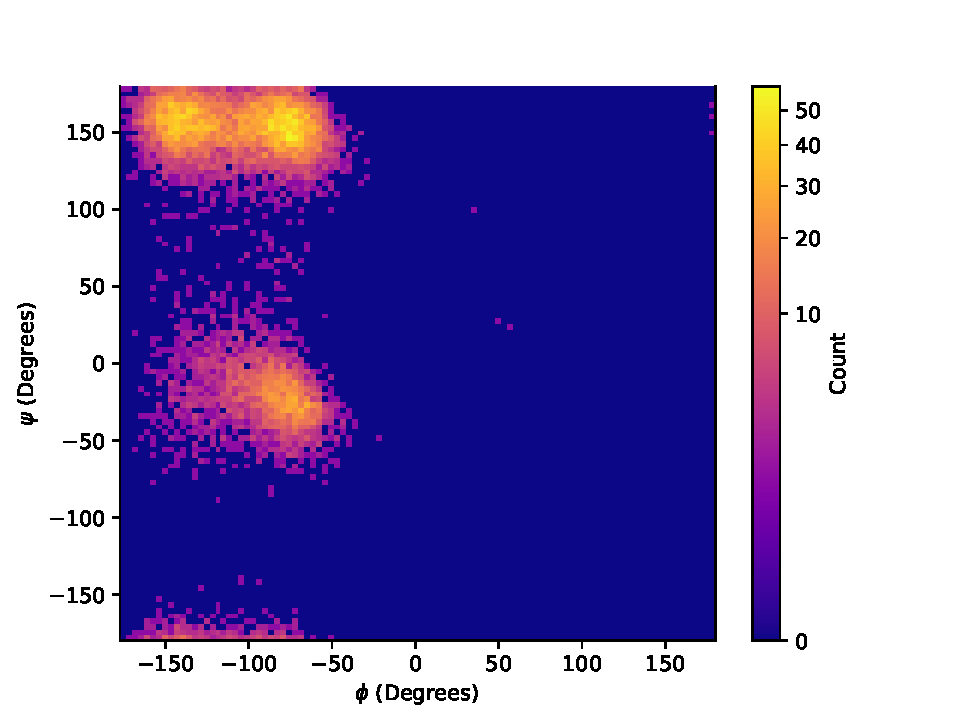
\includegraphics[width=\linewidth]{Figure8.pdf}
\caption{Ramachandran plot showing the occurance of $\phi$/$\psi$ angles of the second peptide bond for each segment throughtout the course of the simiulation.}
\label{fig:view}
\end{figure}
%%%%%%%%

\subsubsection{Conclusion}

Users should now be familiar with setting up a two-dimensional progress coordinate and working with auxiliary data. 
These two tools will help to expand your repertoire of WESTPA simulation techniques and give you access to more complex and informative simulations. 
Users should also now be familiar with changing bin spacings “on-the-fly” as well. 

\subsection{Advanced Tutorial 1: Folding of Chignolin Mini-Protein}

\subsubsection{Introduction}

Protein folding processes have been challenging to simulate due to the relatively long time scales involved. 
In this tutorial, we will use WESTPA to simulate the folding and unfolding of the chignolin mini-protein and to calculate the corresponding rate constants. 
We will run steady-state WE simulations of chignolin folding and unfolding processes separately. 
We will also compare the results of these simulations with those from brute force MD simulations, demonstrating the correctness and potential usefulness of the WE strategy. 
 
\textbf{Learning Objectives.} This tutorial demonstrates how steady state WE simulations can be used to generate pathways and rate constants for both protein folding and unfolding processes.  

Specific learning objectives include:
\begin{enumerate}
\item How to use brute force simulations to identify appropriate initial and/or a target states
\item How to obtain the probability flux into the target state of a WESTPA simulation, how to convert it to a mean rate constant, and how to interpret the results
\end{enumerate}

\textbf{Prerequisites.} Users should have completed the Basic Tutorial.
 
\textbf{Computational Requirements.} We note that significantly more computing time is required for the folding simulations to yield converged rate constants and hence we suggest the user should start with the unfolding simulations. 
In particular, the WE unfolding simulation required \textasciitilde 53 hours for 1000 iterations on 32 CPU cores of 2.6 GHz Intel Xeon processors (\textasciitilde 5 GB of disk space) while the WE folding simulation required \textasciitilde 8 days for 10,000 iterations (200 ns of molecular time) using the same resource (\textasciitilde 50 GB of disk space).
To become familiar with setting up and running the WE simulations, the users can carry out several iterations.  Also, the brute-force simulation described below can be performed for tens of ns, as we benchmarked this system to produce ~150 ns per day on one of the above-mentioned CPUs. Output files for 1000 iterations of the WE unfolding and 10000 iterations of the WE folding simulations (as well as for 4 us of the brute-force simulation) can be found in the corresponding subdirectories. These files should be used for the analysis procedures outlined below.
This tutorial uses AmberTools19’s \verb|sander| package for dynamics propagation and the  \verb|cpptraj| package for progress coordinate calculations (\url{http://ambermd.org/AmberTools.php}). AmberTools is available free of charge.

\textbf{The System.} The chignolin mini-protein with the sequence GYDPETGTWG forms a $\beta$-hairpin and folds/unfolds on a timescale that is accessible to brute force simulations, which provide a reference data set for comparison with WESTPA results. 
The folded chignolin structure (PDB code: 1UAO, \citep{Honda2004}), serves as the starting structure for both the brute-force and WE unfolding simulations. 
Both dynamics propagation and simulation analysis are carried out using the Amber software package. 
Simulations were run at 275 K using the Amber ff14SBonlysc force field \citep{ff} and generalized Born implicit solvent \citep{implicit_solvent}. 

\subsubsection{Brute Force Simulations}

\textbf{Overview.} As mentioned in Section 1.2.1, it is important to run multiple short, brute force simulations prior to using WESTPA. 
In the case of chignolin, which both folds and unfolds on timescales accessible to brute force simulation, brute force simulations can provide information on defining the unfolded and folded states. 
 
\textbf{Running and Analyzing the Brute Force Simulation.} We perform a 4-$\mu$s brute force simulation of chignolin and write out coordinates every 20 ps. 
All files can be found in the \verb|brute_force/| directory. 
The user can change these parameters in the MD config file \verb|md.in|. 
The simulation can be submitted with the following command:
 
\verb|$ ./run.sh|
This submission script may have to be adjusted to the user’s computing platform.

The chignolin C\textsubscript{$\alpha$} RMSD can be computed in the following way:

\verb|$ cpptraj chignolin.prmtop < get_rmsd.in|

This command assumes the brute force simulation trajectory as well as the chignolin parameter topology and folded structure pdb files are all in the current directory.

The output RMSD data file, \verb|rmsd.dat|, lists the time evolution of the chignolin C\textsubscript{$\alpha$} RMSD over the course of the simulation (each line corresponds to a frame). 

Figure 9 shows the C\textsubscript{$\alpha$} RMSD over simulation time for a brute-force simulation that started from the folded $\beta$-hairpin, revealing several unfolding and refolding events within 4 $\mu$s. 
The unfolded and folded states are defined by visual inspection of the RMSD plot and simulated conformations, which show a fully formed $\beta$-sheet and native hydrogen bonds at RMSD < 0.5 \AA{} and a disrupted $\beta$-sheet with broken native hydrogen bonds at RMSD > 4 \AA{} (this pair of RMSD values will also be used later to define target states in WESTPA simulations).  
Note that the (un)folding rate constants will be sensitive to the state definitions, and defining states is a challenging process beyond the scope of this tutorial. 
Our state definitions are designed to avoid potential recrossing artifacts in rate calculations: once a trajectory reaches a state it should tend to remain there, rather than immediately returning to the previous state.
 

%%%Fig 9%%%
\begin{figure}
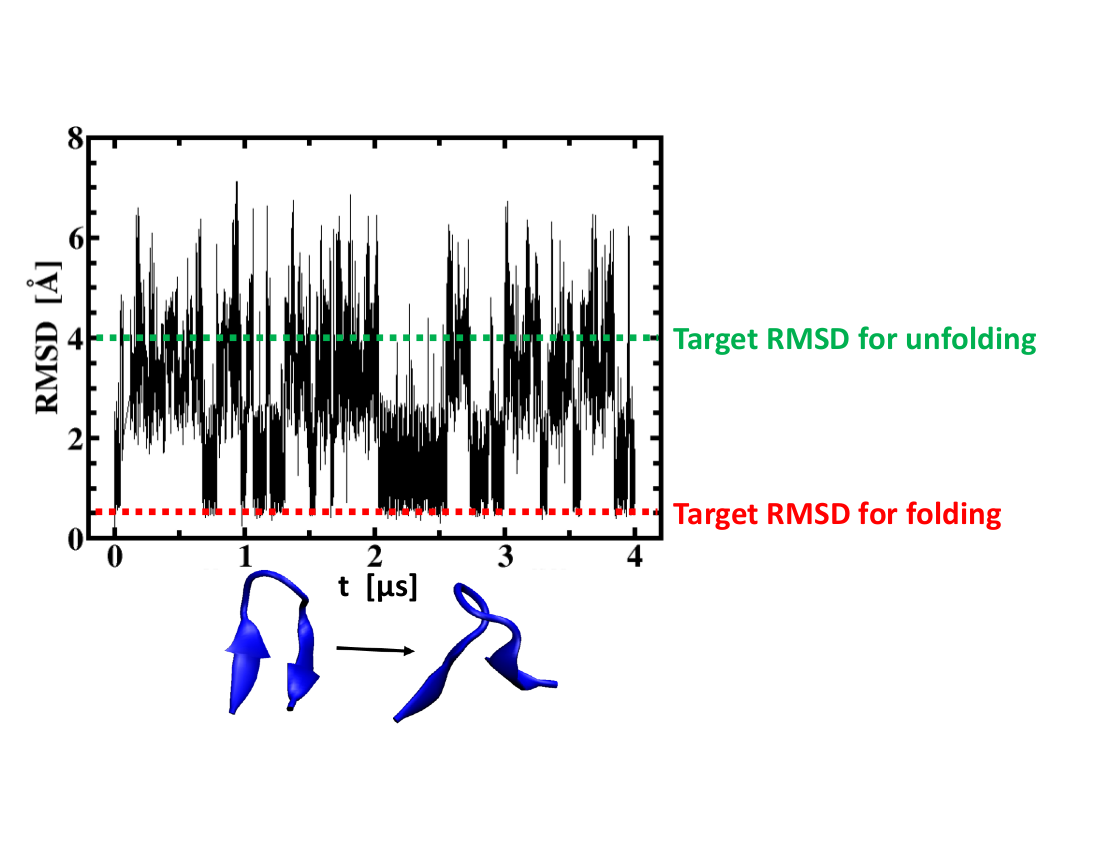
\includegraphics[width=\linewidth]{Figure9.png}
\caption{C\textsubscript{$\alpha$} RMSD vs simulation time for the brute force simulation of chignolin.}
\label{fig:view}
\end{figure}
%%%%%%%%

According to the Hill relation \citep{Hill1989}, the rate constant is exactly the inverse mean first-passage time (MFPT) of the underlying process, where, for instance, the FPT for unfolding is the time required to reach the unfolded state (RMSD > 4 \AA) after first folding(RMSD < 0.5 \AA). 
The user can run the following to obtain the MFPTs for both the folding and unfolding processes: 

\verb|$ python  get_mfpt.py   rmsd.dat   20e-12   0.5   4.0|

The command-line arguments are the RMSD data file, time interval at which the RMSD values are calculated in seconds, and threshold RMSD values for the folded and unfolded states in Angstroms. 
The rate constant of unfolding is estimated to be 0.13 x 108 s\textsuperscript{-1} (confidence interval: 0.09 x 108 s\textsuperscript{-1} – 0.18 x 108 s\textsuperscript{-1}) and that of folding is estimated to be 0.71 x 107 s\textsuperscript{-1} (confidence interval: 0.44 x 107 s\textsuperscript{-1} – 1.24 x 107 s\textsuperscript{-1}). 
Confidence intervals are derived from a Bayesian bootstrapping procedure [Mostofian-2019]. 

\subsubsection{Using WESTPA}

\textbf{Overview.} We will carry out separate steady-state WE simulations for the unfolding and folding processes. 
This strategy is not only more efficient than equilibrium WE simulations in estimating rate constants (see Section 6.1.3), but enables us to set WE parameters for each process (e.g. bin spacing) in a more process-specific way if needed. 
The target state of the folding simulation will be used as the initial state of the unfolding simulation and vice versa. 

\textbf{Choosing an Initial State.} As done for the brute force simulations, WE simulations of the unfolding process will be started from the NMR structure of chignolin WE simulations of the folding process will be started from an unfolded conformation of chignolin (RMSD > 4 \AA) that has been generated by the above brute force simulations.
 
\textbf{Files for Dynamics.} All files are in the \verb|common_files/| subdirectory of either the \verb|WE_folding/| or the \verb|WE_unfolding/| directory.
 
\textbf{Preparing the Simulation Environment.} See this subsection in the Basic Tutorial.
 
\textbf{Equilibrium vs Steady State WE.} Here we will run separate steady state WE simulations of the folding and unfolding processes, defining a target state (\verb|TSTATE_ARGS|) in the \verb|init.sh| files.

\textbf{Progress Coordinate, Binning Scheme and $\tau$ value.} As mentioned above, we will use a one-dimensional progress coordinate consisting of the C\textsubscript{$\alpha$} RMSD from the folded structure of chignolin. 
Although the RMSD with respect to a single reference structure may not be an ideal coordinate for distinguishing between  various conformation, it proves sufficient for our example. 
Folded and unfolded states are defined based on maximum and minimum RMSD values, respectively, that have been sampled by the above brute force simulations. 
We will use a bin spacing  of 0.2 \AA{} and a $\tau$ value of 20 ps. 
However, the very first bin for the unfolding simulations is larger than the regular bin width with RMSD = [0 \AA, 0.5 \AA] because any structure with RMSD < 0.5 \AA{} is considered to be in the folded initial state. 
Analogously, for the folding simulations, the very last bin is larger than the regular bin width of 0.2 \AA. 
  
\textbf{Other WE Parameters.} As done in the above tutorials, our WE simulations were carried out using 4 trajectories/bin. 
The unfolding and folding simulations were run for 1000 and 10,000 WE iterations, respectively, in order to reach a steady value of the corresponding rate constants. 
 
\textbf{Initializing and Running the WE simulations.} The \verb|init.sh| and \verb|run.sh| files can be found in the corresponding directories for both WESTPA simulations. 
The RMSD progress coordinate is calculated and its values returned to \verb|WEST_PCOORD_RETURN|.   

\textbf{Monitoring and Analyzing the WE Simulations.} To compute the rate constant for the folding or unfolding process, we first calculate the mean probability flux into the target state by running the following WESTPA analysis tool:
 
\verb|$ w_fluxanl|
 
The output is the H5 file \verb|fluxanl.h5|, which contains the instantaneous probability flux into the target state at any iteration. 
The following Python script calculates, for any WE iteration, the average rate constant based on the corresponding probability flux arriving in the target state over a preceding window of molecular simulation times (e.g., over 1 ns):
 
\verb|$ python get_mean_rate.py 20e-12  1e-9|

The command-line arguments are the $\tau$ value and the time width for window-averaging. 
Both arguments are in units of seconds.
 
Figure 10 shows the evolution of the average unfolding rate constant of chignolin as a function of molecular time for three independent WE simulations. 
After a few ns, the average rate constants for all of these simulations have leveled off and are roughly comparable to that derived from brute force simulations. 
One difference between the WE and brute force simulations is that the former estimates the MFPT based on the chosen initial structure(s) which may not correspond precisely to the ensemble of starting structures implicit in extracting first-passage events from brute force simulations. 
Note that a three-fold difference in the rate constants among the three WE simulations amounts to only \textasciitilde 0.6 kcal/mol difference in the effective free energy barrier to unfolding (at the simulation temperature of 275 K).

%%%Fig 10%%%
\begin{figure}
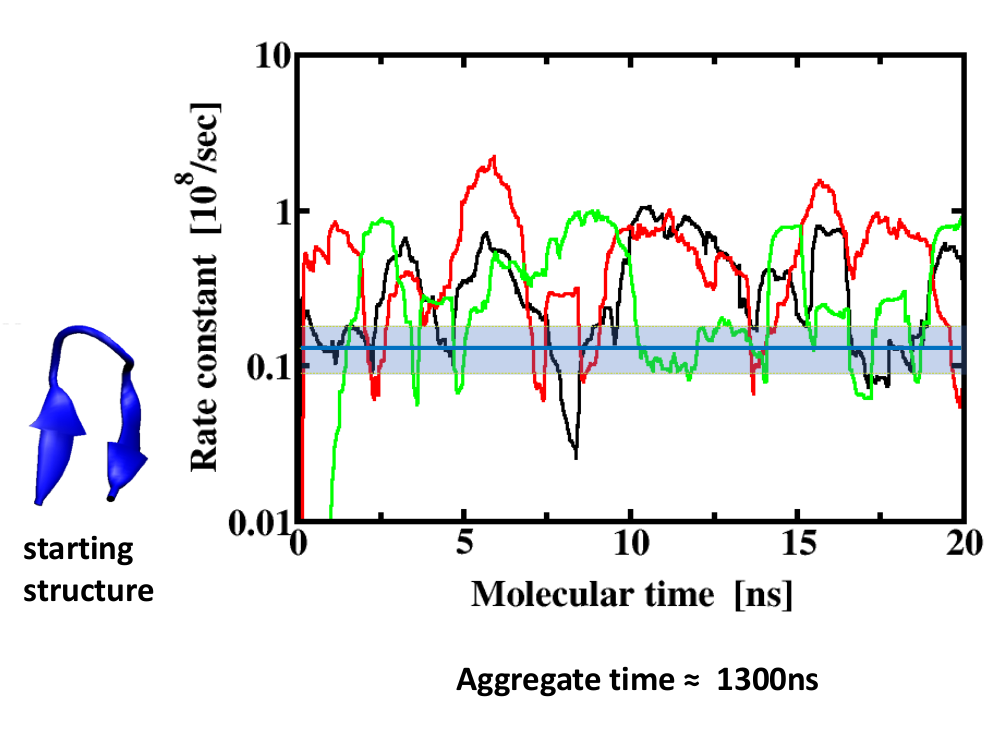
\includegraphics[width=\linewidth]{Figure10.png}
\caption{Estimating the unfolding rate constant of chignolin. 
The 1 ns window-averaged unfolding rate constant is shown in a semi-logarithmic plot for three independent WE simulations (black, red, and green) that were started from the same folded starting structure (see lower left). 
The corresponding unfolding rate constant from the brute force simulation is indicated by the horizontal blue line and its confidence interval by the shaded region. 
The molecular time is the time elapsed, N\textsubscript{$\tau$} where N is the number of WE iterations that each have a length of $\tau$. 
The aggregate simulation time was on average, \textasciitilde 1.3 $\mu$s for each simulation.}
\label{fig:view}
\end{figure}
%%%%%%%%

Figure 11 shows the evolution of the average folding rate constant for chignolin as a function of molecular time for three independent WE simulations. 
Compared with unfolding simulations, the folding simulations require much longer to reach a converged average rate constant that is in rough agreement with that from the brute force simulations; we note that the average rate constant is dominated by the largest flux. 
In addition, the folding rate constant exhibits significantly larger fluctuations, even after the apparent transient period of the first \textasciitilde 100 ns, indicating that the chosen bins are less suited for the folding process. 
During the folding process, distinct hydrogen bonds must be formed between the neighboring anti-parallel strands, and possibly in a specific order, to eventually reach an RMSD < 0.5 \AA. 
In contrast, the unfolding process results in faster convergence of the corresponding rate constant and likely involves the simultaneous breaking of hydrogen bonds in order to reach an RMSD > 4 \AA.

%%%Fig 11%%%
\begin{figure}
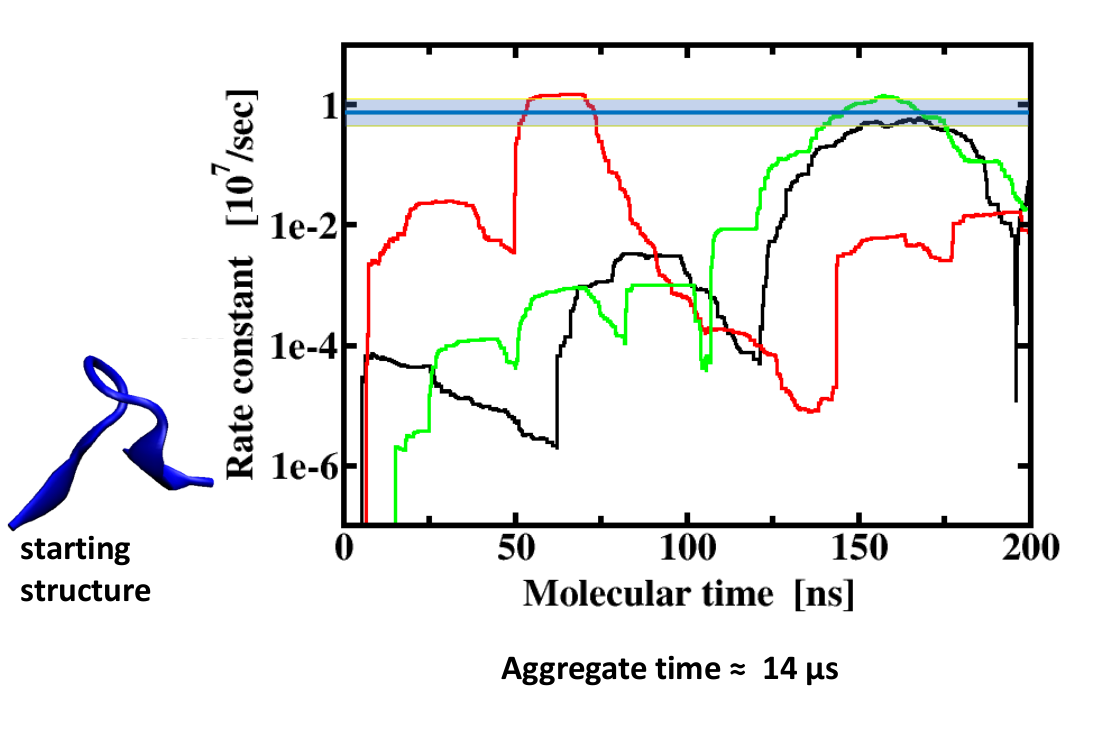
\includegraphics[width=\linewidth]{Figure11.png}
\caption{Estimating the folding rate constant of chignolin. 
The 20-ns window-averaged folding rate constant is shown in a semi-logarithmic plot for three independent WESTPA simulations (black, red, and green profiles) with the same unfolded starting structure (see lower left). 
Note the significantly longer molecular and aggregate simulation times for each simulation to obtain converged rates of folding compared to unfolding (see Figure 11). 
The corresponding rate constant from the brute force simulation is indicated by the horizontal blue line and its confidence interval by the shaded region.}
\label{fig:view}
\end{figure}
%%%%%%%%

The resulting WE simulations consist of multiple continuous unfolding or folding pathways that may cover different regions of configurational space at any given time. 
To select for particular pathways (trajectories), we can run the following: 
 
\verb|$ python get_target_trajs.py  1  10000|

The command-line arguments indicate the first and last iteration number to be considered. 
The output file \verb|target_trajs.dat| has two columns: one with the iteration number and one with the segment number of the trajectory that has reached the target state at that iteration. 
Thus, the number of rows indicates the total number of generated events. 
The iteration and segment numbers can be used by \verb|w_trace| to obtain the full path of a particular folding or unfolding event (see Section 6.1.6).

\subsubsection{Conclusion}

In this tutorial, you have learned how to apply the WE strategy to simulate a protein folding process under steady state conditions. 
The recycling of trajectories at a target state allows the generation of a non-equilibrium, steady state, to which the trajectory ensemble converges faster compared to an equilibrium ensemble of trajectories. 
Such steady states trajectories enable  the direct computation of rate constants as described in this tutorial.   

\subsection{Advanced Tutorial 2: K\textsuperscript{+}/18-Crown-6 Ether Dissociation with the WExplore Plugin}

\subsubsection{Introduction}

For many biomolecular systems, it can be difficult to capture all of the slow motions in one or two collective variables. 
This can hinder sampling of the events of interest. 
The WExplore algorithm was developed to perform weighted ensemble sampling in a many-dimensional space by using a hierarchical binning scheme of Voronoi polyhedra. 
This allows a user to broadly explore the dynamics of their system of interest along many dimensions, starting from only a single initial structure.

The key quantity to enable this is a distance metric: a way of measuring the distance between two trajectories at a given point in time. 
In order to assign a given trajectory, $X$, to a region, this metric is used to calculate the distance from $X$ to a set of “images” that define the Voronoi polyhedra. 
The trajectory $X$ is then assigned to the region whose image has the smallest such distance. 
To efficiently assign trajectories to regions in a high-dimensional space, a hierarchy of regions is employed: a small set of very large regions tile the full space, each of which are tiled by a set of smaller regions, which are themselves tiled by smaller regions, and so on. 
The WESTPA-WExplore plugin defines the hierarchical regions on-the-fly; assigns trajectories to regions; and balances trajectories between the hierarchical regions. 
The user only needs to define the distance metric appropriate for their system and set a few parameters of the algorithm.

\textbf{Learning Objectives.} This tutorial covers the installation and use of the WESTPA-WExplore plugin for a simple system: the dissociation of a K\textsuperscript{+} ion from 18-crown-6 ether.

Specific learning objectives include:
\begin{enumerate}
\item How to install and use the WExplore-WESTPA plugin
\item How to define and implement a distance metric for use in WExplore simulation
\item Determining appropriate values for WExplore-specific parameters for a system of interest
\item Analyzing simulations by inspecting properties of the Voronoi “images” 
\end{enumerate}

Users with some WESTPA experience should be able to successfully apply WExplore to their system of interest using their own customized distance metric.

\subsubsection{Prerequisites}

Users should have completed the WESTPA tutorials above on Na\textsuperscript{+}/Cl\textsuperscript{-} and the p53 peptide. 
Users should have an understanding of the WExplore algorithm: how the region hierarchy is defined; how it progressively discovers regions; and how the hierarchical balancing algorithm works. 
Details of the algorithm can be found in previous work \citep{Dickson2014}. 

\textbf{Computational Requirements.} This tutorial requires 500 MB disk space. 
This simulation takes \textasciitilde 1.5 hours of wall clock time to complete (50 iterations) using 8 threads of a 4 GHz Intel Core i7 processor.  
This tutorial uses Gromacs 2016.2 for dynamics propagation and progress coordinate calculations (\url{http://www.gromacs.org/}).  
Gromacs is available free of charge.

\subsubsection{Installation and Configuration of the WESTPA-WExplore Plugin}

It is necessary to install some other Python packages that you might not need for standard WESTPA simulations. 
We recommend using an Anaconda environment and installing the packages as follows:

\verb|$ conda create -n WESTPA-WExplore westpa scipy|

\verb|pandas networkx|

\verb|$ conda activate WESTPA-WExplore|

Note that if you are running your WESTPA simulations on remote nodes, you would have to include the \verb|conda activate| command in your \verb|env.sh| file. 
To install the plugin, clone the WESTPA-WExplore repository to a location on your computer:  

\verb|$ git clone https://github.com/ADicksonLab/|

\verb|WESTPA-WExplore.git|

This will copy files to your machine, located in the \verb|WESTPA-WExplore/| directory. 
Change to this directory and install the plugin as follows:

\verb|$ cd WESTPA-WExplore/|

\verb|$ python setup.py install|

To test this, go to another directory, and type:

\verb|$ python -c 'import westpa_wexplore'|

If this runs without an import error, then you are ready to proceed to the next step! 

\subsubsection{Preparing the Simulation}

\textbf{The System.} This tutorial will use a simple ligand-binding test system: the dissociation of a K\textsuperscript{+} ion from the 18-Crown-6 Ether molecule (Figure 12), as studied previously \citep{Zwier2011}. 
The goal is to efficiently sample the dissociation of the complex. 
This is reminiscent of applications of WExplore to more difficult ligand dissociation problems, such as the unbinding of the TPPU ligand from soluble epoxide hydrolase, a process with a mean first passage time of 11 minutes \citep{Lotz2018}.

%%%Fig 12%%%
\begin{figure}
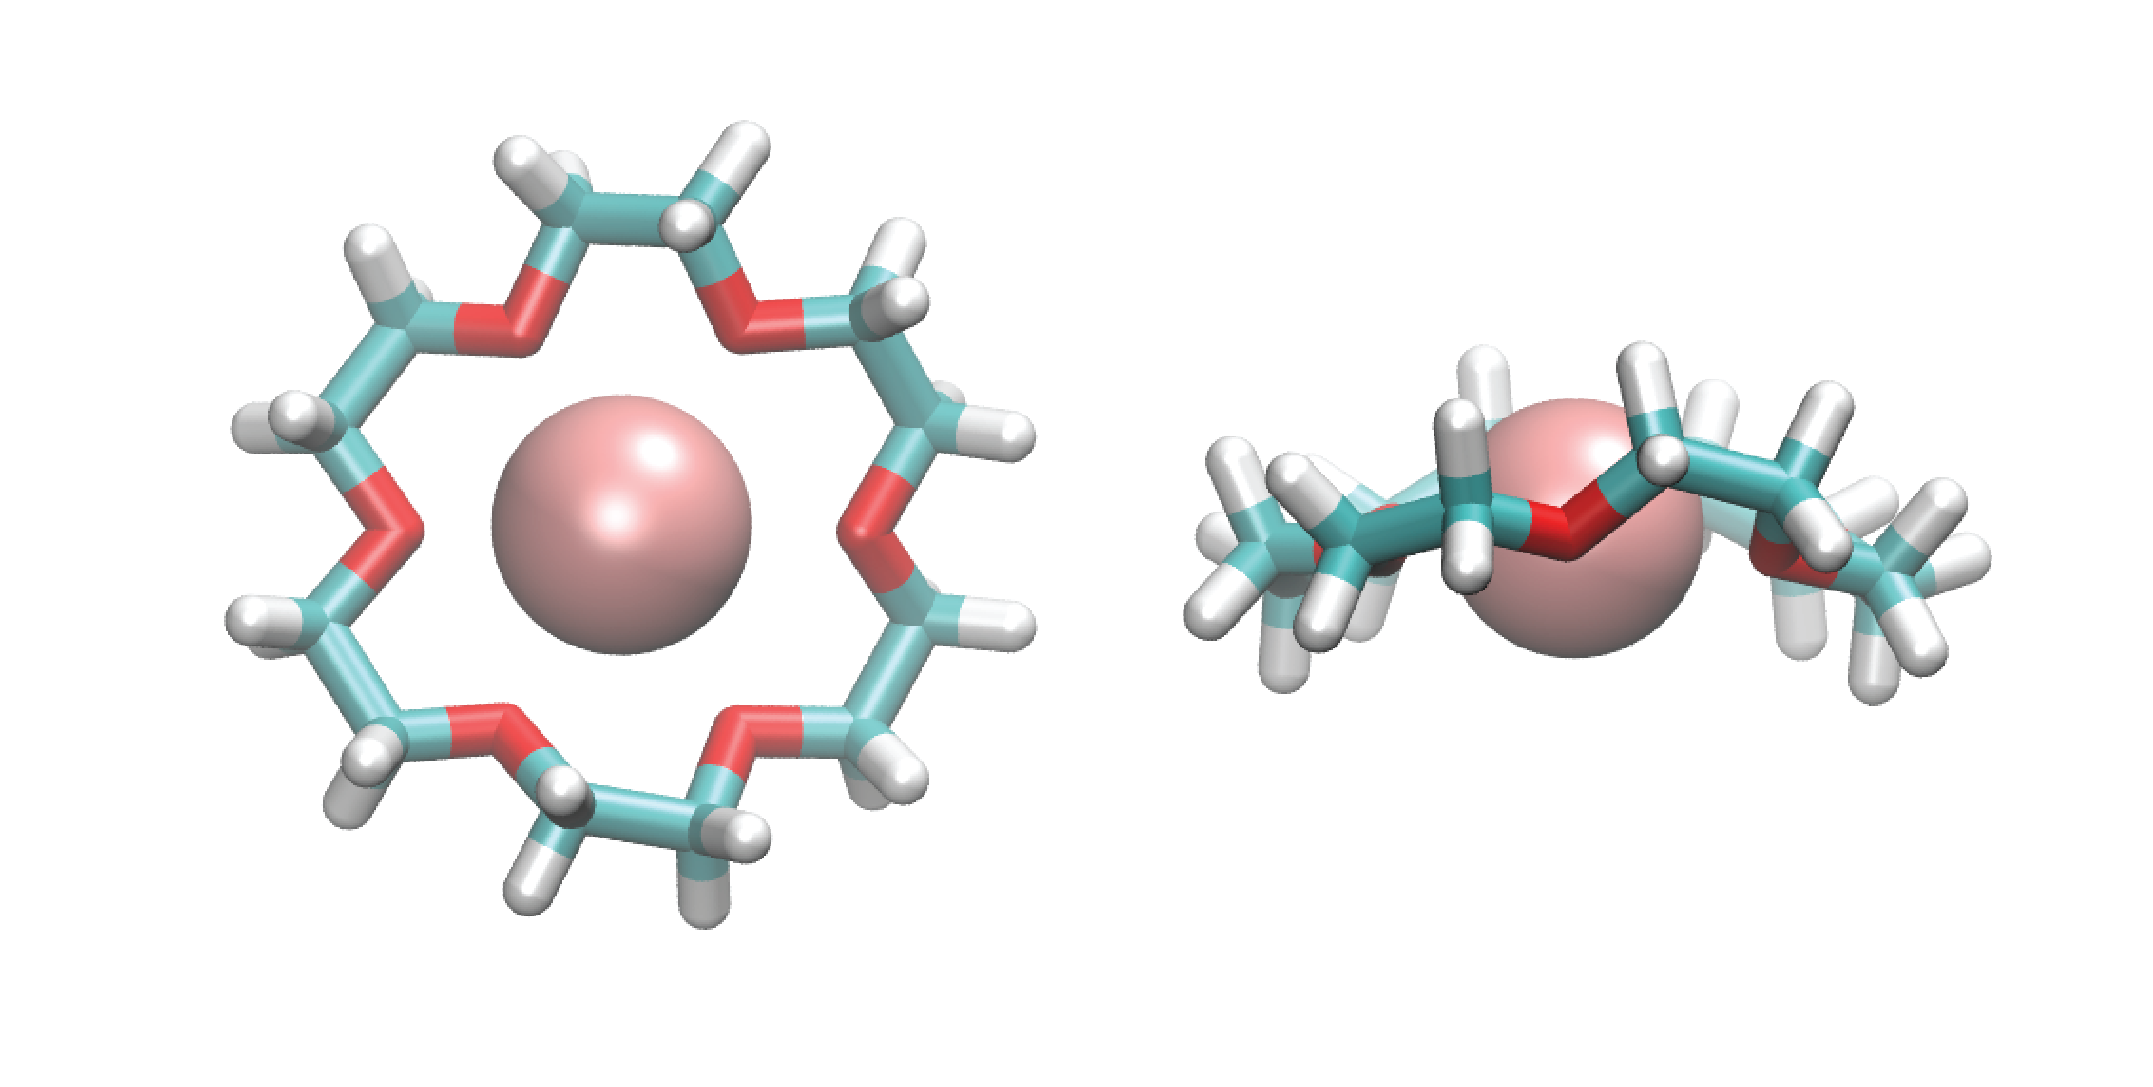
\includegraphics[width=\linewidth]{Figure12.png}
\caption{The K\textsuperscript{+}/18-Crown-6 ether system. 
The K\textsuperscript{+} ion is shown as a pink sphere. Left: top view. Right: side view.}
\label{fig:view}
\end{figure}
%%%%%%%%

\textbf{Distance Metric.} Here we will use a common distance metric for ligand release processes: the root mean squared distance of the ligand atoms after alignment to the host binding site \citep{Dickson2017,Dixon2018,Dickson2018}.
This captures ligand translation with respect to the binding site, and (for systems with more complicated ligands) captures ligand rotation as well as internal degrees of freedom. 
The information needed to calculate these distances is the x, y and z positions of the ligand atoms after alignment to the host molecule. 
The first step to assign a walker to a region, then, is to extract this data from the simulation. 
This is done by a familiar script: \verb|get_pcoord.sh|.

The \verb|get_pcoord.sh| script included in the tutorial repository uses a series of BASH commands to align a crown ether molecule to a reference structure (named \verb|bound_state.tpr|), and then extracts only the lines that contain the ligand atoms, saving them in the file indicated by the \verb|WEST_PCOORD_RETURN| environment variable. 
This data is then processed by the \verb|pcoord_loader| function in the \verb|system.py| file, where the x, y and z data are collected from columns 5, 6 and 7 of the PDB-formatted file. 

This pipeline is rather crude, but effective. 
Note that any set of commands that can extract the output you need (typically, atomic positions) from your simulation output files will do, but it is necessary that changes that you make to \verb|get_pcoord.sh| (which writes to \verb|WEST_PCOORD_RETURN|) are compatible with any changes you make to \verb|pcoord_loader| (which reads from \verb|WEST_PCOORD_RETURN|). 
For instance, one could avoid PDB files all together, and load final structures into the \verb|pcoord_loader| using the Python interface of Amber or Gromacs.

The next step is to define a function that returns the distance between two pcoord vectors. 
This is typically a Euclidean distance, but can be defined in an arbitrary fashion. 
It need not be differentiable, or even continuous, to be effective in a WExplore simulation. 
The distance function is defined by \verb|eucl_dist| in \verb|system.py| and is passed as an argument to the \verb|WExploreBinMapper| function upon initialization of a System object.

\textbf{Setting parameters.} The set of WExplore-specific parameters were discussed above in Section 3.1. 
Most of these are set in the \verb|system.py| file. The sizes of the hierarchical Voronoi polyhedra are set using a list, passed to the \verb|d_cut| argument of the \verb|WExploreBinMapper| function. 
This list should go from largest to smallest, where the number of elements is the same as the number of levels to the hierarchy. 
Similarly, the branching factor is set by a list that is passed to the \verb|n_regions| argument of \verb|WExploreBinMapper|. 
The number of total trajectories is set by the \verb|max_replicas| attribute of the system.

\textbf{Choosing an Initial State.} It is also necessary, upon initializing the system object in \verb|system.py|, to define the initial “image” that corresponds to the first structure used in the simulation. 
This is done in lines 35-37 of the \verb|initialize| function in \verb|system.py| and should be changed as necessary for a given system. 
The initial PDB file containing the aligned K\textsuperscript{+} coordinates was prepared from the basis state 0 (in bstates/0) using Gromacs in the \verb|init.sh| script. 
As described in \verb|BASIS_STATES.single|, we are initializing all trajectories from a single starting structure (“bound\_0”) that has probability = 1.

\textbf{Other parameters.} Other details of simulation parameters are given in the \verb|md.mdp| file. 
For instance, the dynamics timestep (0.002 ps), the number of steps per cycle (1000) and the output frequency for coordinates, velocities and forces (100, 100 and 0, respectively). 
Note that here we are outputting our coordinates 11 times per cycle (1000 / 100, plus one extra for the endpoint). 
This must be consistent with the parameter \verb|pcoord_len| in \verb|system.py|, which is also set to 11 in our case.

\textbf{Preparing the Simulation Environment.} As discussed previously, make sure to modify the env.sh file to reflect the installation locations of WESTPA, Gromacs, etc. on your machine. 
Additionally, add the location of the WESTPA-WExplore package to your \verb|WEST_PYTHONPATH|, e.g.:

\verb|export WEST_PYTHONPATH=/your/installation/|

\verb|location/WESTPA-WExplore/westpa_wexplore:|

\verb|$WEST_PYTHONPATH|

\subsubsection{Running the Simulation}

First we need to initialize the simulation:

\verb|$ ./init.sh|

And then we can run a job. 
This can be submitted to a cluster (we will not go over that here), or run locally, as follows:

\verb|$ ./run.sh --parallel --n-workers 8|

This is a good time to break for lunch. 
In our hands, this will take about 90 minutes on a 4 GHz Intel Core i7 processor.

\subsubsection{Analyzing the WExplore Simulations}

Aside from the way that resampling is implemented, WExplore simulations can be treated just like other WE simulations in terms of analysis. 
All of the techniques discussed above regarding the definition of observables and plotting of probability distributions can be used for WExplore simulations as well. 
Here we will briefly go over how to analyze simulation properties that are unique to WExplore. 
Specifically, the location of the “images” used to define the Voronoi polyhedra.

Firstly, during run time it can be helpful to keep an eye on the number of regions defined so far at each level of the hierarchy. 
A brief report is written, each cycle, in \verb|west.log|:

\verb|--wexplore-stats--------------------|

\verb|wallclock time: 0.221 s|

\verb|Level 0: 10 cells (10 max)|

\verb|Level 1: 69 cells (100 max)|

\verb|Level 2: 193 cells (1000 max)|

\verb|------------------------------------|

\verb|Iteration wallclock: 0:01:41.246056,|

\verb|cputime: 0:12:40.570392|

This is taken from the end of our simulation, where we have defined 10 regions at the largest level of the hierarchy (here, they are at least 5 \AA{} apart), 69 total regions at the medium level (some of which are under the first large region, some under the second, and so on), and 193 total regions at the smallest level. 
It is completely fine if these numbers do not approach their maximum values. 
In contrast, if regions are defined too quickly – especially at the smallest level – then this is a sign that they are too small.  
The log file also displays the wall clock time for the WExplore resampler (0.221 s), which is negligible compared with the total wall clock for the cycle (1 minute, 41 s), as is typical.

The details about the WExplore regions are stored in \verb|west.h5|, along with the positions and progress coordinates. 
The included Python script (\verb|WExplore_analysis.py|) shows how the coordinates of the images can be accessed from the \verb|west.h5| file and analyzed using Python tools like \verb|numpy| and \verb|MDTraj| \citep{mdt2015}.

\subsubsection{Conclusion}

Users should now have everything they need to use the WExplore resampling algorithm on their own system of interest.  
WExplore is a powerful way to generate heterogeneous sampling on energy landscapes that are both rough and high-dimensional. 
The ability to write your own distance metric using tools in python opens up many possibilities. 
For example, a number of dimension reduction tools in sklearn could be easily imported and used to automatically identify a space of collective variables.  

\subsection{Advanced Tutorial 3: Analysis Tools}

In this tutorial, we will go over how to (i) calculate progress coordinates using external analysis suites, (ii) automate analysis of a WE simulation using the WESTPA \verb|w_ipa| tool, and (iii) visualize the evolution of WE datasets with time. 
We focus on the p53 peptide system described above in the Intermediate Tutorial (Section 6.2) in which the progress coordinate is the C\textsubscript{$\alpha$} RMSD of the peptide from its folded, $\alpha$-helical conformation

\subsubsection{Calculating Progress Coordinates Using External Analysis Suites}

\textbf{Introduction.} Here we will demonstrate how to write scripts for calculating custom progress coordinates for WESTPA simulations using the external analysis suites, MDTraj and MDAnalysis \citep{mda2011,mda2016,mdt2015}. 
A prerequisite to this tutorial is completion of the Basic Tutorial. 
You will also need to install the MDTraj or MDAnalysis analysis suites. 
Other required files are provided on GitHub.

\textbf{Learning Objectives.} The specific learning objective of this tutorial is to calculate progress coordinates using an external analysis suite (MDAnalysis or MDTraj). 

\textbf{Explanation of Files and Scripts.} The master configuration file for the simulation, \verb|west.cfg| specifies the dimensionality of the progress coordinate (\verb|pcoord_ndim|), as well as how many progress coordinate data points should be returned from each segment (\verb|pcoord_len|) (it specifies many other things but these are of primary interest for this tutorial as they specify the shape of the progress coordinate).

The script \verb|rmsd.py| is responsible for using MDTraj or MDAnalysis to calculate the RMSD values during the simulation. 
Read the comments in the script to understand its setup for each package (there is a unique version for both).

Two scripts are responsible for calling \verb|rmsd.py| at different points in the simulation (both found in \verb|westpa_scripts/|):
\begin{itemize}
\item \verb|get_pcoord.sh| calculates the progress coordinate during the initialization of the system. 
Because dynamics have not been run yet, WESTPA only needs a single point progress coordinate, rather than an array. 
This difference is controlled by the FORM argument, explained in the \verb|rmsd.py| script.
\item \verb|runseg.sh| calculates the progress coordinate during dynamics propagation. 
It passes each segment's trajectory file as input to the custom progress coordinate loader, \verb|rmsd.py|.
\end{itemize}

There are slight differences in these files for the MDAnalysis and MDTraj setups, explained in the comments of each script.

\textbf{Files in amber\_config/ directory:}
\begin{itemize} 
\item \verb|P53.MDM2.prmtop| - The topology file.
\item \verb|md.in| - The input file which specifies conditions for dynamics propagation.
\end{itemize}

The other files needed for the simulation are found in the bstates folder, and are explained in the MDAnalysis/MDTraj specific sections below.

\textbf{Running the Simulation.} Before running the simulation, you may want to change the binning scheme, the number of iterations, or other parameters, which can be found in \verb|west.cfg|.

To run the simulation, only two scripts must be executed. To initialize the system:

\verb|$ ./init.sh|

To run the simulation in the background:

\verb|$ ./run.sh &|

To monitor the progress of the simulation:

\verb|$ tail -f west.log|

The rest of the tutorial is specific to the software package used. 
See below for specifics involving the MDAnalysis and MDTraj analysis suites.

\textbf{Using the MDAnalysis Analysis Suite}

Files in \verb|bstates/| directory:
\begin{itemize}
\item \verb|P53.MDM2.rst| - Used as initial crystal structure to compare to the trajectory when calculating the RMSD and to start new trajectories in \verb|runseg.sh|.
\item \verb|bstates.txt| - specify restart file \verb|P53.MDM2.rst|.
\end{itemize}

\textbf{Using the MDTraj Analysis Suite}

Files in \verb|bstates/| directory:
\begin{itemize}
\item \verb|P53.MDM2.nc| - because MDTraj does not support restart files, this file is used in \verb|get_pcoord.sh| to calculate the initial progress coordinate. 
It is also used by \verb|runseg.sh| as an initial crystal structure to compare to the trajectory when calculating the RMSD.
\item \verb|P53.MDM2.rst| - Used to start new trajectories in \verb|runseg.sh|.
\item \verb|bstates.txt| - specify restart file \verb|P53.MDM2.rst|.
\end{itemize}

\textbf{Conclusion.} You have learned in this tutorial the basic structure of a Python script to calculate progress coordinates for WESTPA using the MDAnalysis and MDTraj analysis suites. 
There are two scripts run by WESTPA which call \verb|pcoord_loader.py|, triggering the calculation of progress coordinates. 
The bash script, \verb|get_pcoord.sh|, triggers the calculation of only a single progress coordinate, while \verb|runseg.sh| triggers the calculation of the progress coordinate at multiple points in a trajectory, as defined in \verb|west.cfg|. 
It is important to include the last line of the Python scripts, setting \verb|segment.pcoord| equal to the progress coordinate array, so that the progress coordinate may be used to further the simulation.

\subsubsection{The w\textunderscore ipa Analysis Tool}

\textbf{Introduction.} The \verb|w_ipa| analysis tool is designed to facilitate analysis of WESTPA simulation datasets through a single interface (Jupyter Notebooks or the command line). 
In particular, \verb|w_ipa| automates analysis routines, ensures data consistency through the use of automatically updated “analysis schemes”, enables a user to easily view a particular dataset or trajectory segment in the H5 file, and monitors the progress of the simulation (e.g. trajectory weights, progress coordinates, and other properties of interest).  

Learning Objectives. The specific learning objectives of this tutorial are to use the \verb|w_ipa| analysis tool to:
\begin{enumerate} 
\item Calculate rate constants
\item Trace and analyze trajectory segments (weight, pcoord, auxdata)
\item Plot datasets
\end{enumerate}

\textbf{Setting Up.}  Using \verb|w_ipa| is straightforward. 
The \verb|west.cfg| file, which specifies most of the simulation parameters, also specifies the analysis parameters under the \verb|Analysis| heading.

The general format of the analysis section can be seen in the included \verb|west.cfg| file. 
More detailed examples are available in the Basic and Intermediate Tutorials.

In order to run \verb|w_ipa|, there must be at least a single analysis scheme specified. 
This scheme does not have to consist of the bins and/or state definitions used during the simulation. 
Less physically relevant schemes may be employed. 
Any changes made to analysis schemes in the \verb|west.cfg| file will be actualized the next time \verb|w_ipa| is run. 
The user is therefore guaranteed to never wonder whether the analysis files are up to date. 

The \verb|assign.h5|, \verb|reweight.h5|, and \verb|direct.h5| files are stored under \verb|ANALYSIS/SCHEME_NAME|.
The optional arguments that can be passed to \verb|w_assign|, \verb|w_direct|, and \verb|w_reweight| can be specified by creating a section with the tool name and using the value pairs argument. 

\textbf{The Interface}. To run \verb|w_ipa| from the command line, enter the command \verb|w_ipa| after having sourced \verb|westpa.sh| (if not already sourced). 
To run \verb|w_ipa| in a Jupyter notebook enter the command \verb|w_jupyter| from the command line. 
When you create a new Jupyter notebook, there are some basic Python commands that must be executed:

\verb|import w_ipa|

\verb|w = w_ipa.WIPI()|

\verb|# At startup, it will load or run the analysis|

\verb| schemes specified in the configuration file|

\verb| (typically west.cfg)|

\verb|w.main()|

\verb|w.interface = 'matplotlib’|

The Python kernel must be launched with the use of \verb|w_jupyter|, or otherwise, the \verb|$PYTHON_PATH| variable must be set to include the WESTPA directories. 
The command \verb|w_env|, which ships with WESTPA, is responsible for setting environment variables and can be used with the jupyter notebook command to ensure \verb|w_ipa| is importable.

All commands are applicable from both the command line and Jupyter notebook interface; if plotting functions are called from the command line, the plot will appear within the console (it can be configured to use matplotlib if desired; this requires an active, available X session).

All of the variables are now accessible from the \verb|w| object.

\textbf{Changing Schemes and Accessing Datasets.} A typical analysis routine begins by selecting an appropriate analysis scheme that may consist of multiple state definitions, averaging options, or reweighting parameters that are appropriate for the simulation. 
Most of the datasets are presented from the current, “active” state, although access to other datasets is conveniently available. 
All numerical datasets are given as numpy arrays, allowing for easy analysis of data.

To see what schemes are available, run the following command:

\verb|$ w.list_schemes|

To change schemes, you may set the \verb|w.scheme| variable to a string or integer value (corresponding to the index of the scheme). 
For instance, suppose you have the following two schemes: “\verb|EXAMPLE|”, and “\verb|ALTERNATE|”, and the current scheme is "\verb|EXAMPLE|". 
To access the properties of the current iteration in the current scheme (explained in more detail below), you would type the following:

\verb|$ w.current|

However, to access the alternate scheme, you would run the following command:

\verb|$ w.schemes.ALTERNATE.current|

Where “\verb|ALTERNATE|” corresponds to the scheme name written in the \verb|west.cfg| file.

The \verb|w_ipa| tool works by presenting an iteration and all its data as a single object. Each iteration object contains numerous datasets and helper functions designed to ease analysis. 
After loading, \verb|w_ipa| defaults to the final iteration. 
You can change the iteration by using the following command: 

\verb|$ w.iteration = 39|

At any time, we have three iteration objects available in the object ‘\verb|w|’: current, past, future. 
The past and future datasets are keyed to the parents and children of the segments in the current dataset. 
For instance, if you are analyzing segment 200 in the current iteration and wish to analyze the parent segment it came from, you could access the two datasets using the following iteration objects:

\verb|$ w.current[200]|

\verb|$ w.past[200]|

Even though it is very unlikely that the actual segment ID of the parent of segment 200 is 200, it is mapped correctly to enable convenient analysis. 
To obtain the actual segment ID, just run:

\verb|$ w.past[200].seg_id| OR \verb|w.past[200][‘seg_id’]|

As indicated above, objects in \verb|w_ipa| can be called either as Python dictionaries or as attributes on the object. 
These can be listed by calling the print method on the parent object. 
In addition, as \verb|w_ipa| is using iPython under the hood, tab completion works as when using the command-line interface (CLI).

To access the main datasets of interest, \verb|pcoord| and \verb|auxdata|, type the following: 

\verb|$ w.current.pcoord|

\verb|$ w.current.auxdata|

These commands will output the full datasets, which can be useful for calculating properties on all trajectory segments at once. 
But what if we are only interested in looking at the properties of particular segments?

You could manually find a segment of interest, but \verb|w_ipa| includes a few convenient properties that return certain segments. 
In particular, \verb|w.current| provides the following:

\verb|maxweight|

\verb|minweight|

\verb|successful_trajectories|

The \verb|maxweight| and \verb|minweight| properties return objects which contain data about the segments that carry the highest and lowest weights in the current iteration, respectively. 
The \verb|successful_trajectories| property returns the IDs of the segments that successfully transitioned between states  (the states are defined in your \verb|west.cfg|). 
Calling these functions on aniteration object yields all datasets pertaining to the segment with the desired property. 
In this WE simulation, each trajectory contains 101 timepoints. 
Therefore, the \verb|maxweight| segment (seg\_id 177) in iteration 49 has (101,2) pcoord values, 101 auxdata values, and it can switch bins and states 101 times. 
You can see this by running \verb|w.current.maxweight|.
 
The \verb|auxdata| dataset is unique in that the simulations can contain any number of auxiliary datasets with any unique name. 
Here, they are returned as a dictionary where the key: value pair is the dataset name defined in \verb|west.cfg|, and the value is a numpy array containing the actual dataset.

Segment 177 above was in state 1 during the entire iteration. 
But what is state 1? 
It is defined in \verb|west.cfg|, but we do not have to go back to \verb|west.cfg| to look it up. 
Simply run:

\verb|$ w.state_labels|

It is also in bin 0 the entire time (note that these are the bins defined in \verb|west.cfg| for this analysis scheme and not the bins used in the simulation). 
What is the pcoord value of that bin? Run:

\verb|$ w.bin_labels|

To track the immediate parent and children of a segment, we can use \verb|w.past| and \verb|w.future|. 
These iteration objects are similar to \verb|w.current|, but keyed to give information about the segments in \verb|w.current|. 
For instance, to look up the weight of segment 177’s parent, run the following:

\verb|$ w.past[177].weights|

Likewise, to see whether the same segment had any children, run:

\verb|$ w.future[177]|

Segments always have a past, but do not always have a future. 
They may also produce multiple children, so the values returned by \verb|w.future[seg_id]| are usually more complicated. 
Rather than being given the datasets directly, \verb|w.future| returns a list of the datasets.

To determine the properties of a complete trajectory (that is, the string of segments going back to the first iteration), \verb|w_ipa| includes a fast trace function. 
To trace segment 177 in iteration 39 (current iteration), run the following:

\verb|$ s = w.trace(177)|

It returns an object similar to \verb|w.current[177]|, except that it also contains all historical information. 
The \verb|auxdata|, \verb|bins|, \verb|pcoord|, and \verb|states| datasets are all going to be very large; their shape should be the product of the number of timepoints per iteration and the trajectory length. 
As we are at iteration 39, and have 101 time points per $\tau$ value, we should have 3939 values in each dataset! 

\textbf{Plotting.} Rather than visually inspecting each value, let us just plot it. 
Run the following:

\verb|$ clear|

\verb|$ s.weights.plot()|

\verb|$ clear|

\verb|$ s.pcoord.plot()|

\verb|$ clear|

Many datasets, such as \verb|weight|, default to a logscale; others, such as \verb|pcoord|, use a linear scale. 
By default, the 0th dimension of \verb|pcoord| is plotted. 
When the plotting function is called via the CLI, a rough estimate of how the trajectory’s pcoord has evolved is plotted in the terminal.

The \verb|w.current| iteration object contains information about the rate constants that were calculated in the active analysis scheme. 
To view an array containing the rate constants along with the upper and lower confidence intervals, run the following (do not forget about tab completion): 

\verb|$ w.current.direct.rate_evolution| OR \verb|$ w.current.rate_evolution.direct|

To view a plot of their evolution, run the following:

\verb|$ w.current.direct.rate_evolution.plot()|

The \verb|w_ipa| tool displays the upper and lower confidence intervals on the plot as well. 

\subsubsection{Visualization of WE Datasets}

In addition to generating probability distributions as a function of the progress coordinate (or other observables of interest), it can be helpful to examine movies of how the distributions evolve with time. 
Such movies can be used to determine the optimal number of trajectories/bin in a particular region of the progress coordinate by tracking how the probability distribution evolves with the number of trajectories that region. 

\textbf{Learning Objectives.} The specific learning objectives of this tutorial are:
\begin{enumerate}
\item Create a movie of how a probability distribution evolves with time.
\item Trace representative trajectories over this probability distribution.
\end{enumerate}

Here, we will create a movie of how a two-dimensional probability distribution (Figure 13) evolves with time. 
This movie-making feature is currently carried out using a bash script (\verb|pdist_evol.sh|) and will eventually be added to the WESTPA \verb|plothist| tool. 

The bash script involves the following three steps: 1) run the \verb|w_pdist| tool on the \verb|west.h5| file to generate probability distributions in a specified folder that will also contain the eventual movie of how the distributions evolve with time, 2) generate a plot of a two-dimensional probability distribution for each iteration as a cumulative moving average from iteration 1 to 40, and 3) create the movie from the 40 generated frames of the probability distributions. 
The most important part of this script is the \verb|--postprocess-function| option of \verb|plothist| that is defined in \verb|postprocess.py|. 
This function requires a basic knowledge of Python and \verb|matplotlib|, and can be used to modify features of the plot (e.g. adjustment of axis labels, tick marks, titles, and lines) via the \verb|matplotlib| interface. 
In addition, external files from various analyses can be uploaded and overlaid on the plot as demonstrated in this example. 

Here, we will select two trajectories from the last WE iteration and overlay their pathways on the probability distribution of the overall simulation as a function of progress coordinate. 
First, we will use the \verb|trace_walker| function to determine the segment number of the selected trajectories in each WE iteration going all the way back to the corresponding conformation of the initial state ensemble. 
This process of tracing can also be accomplished by using WESTPA tools \verb|w_ipa| and \verb|w_trace|. 
After the segment numbers are obtained, the \verb|get_pcoords| function loads in 10 progress coordinate values per iteration for the trajectories. 
Finally, a movie-making tool (here, we use \verb|mencoder|) creates a movie from the 40 frames of probability distributions. 

%%%Fig 13%%%
\begin{figure}
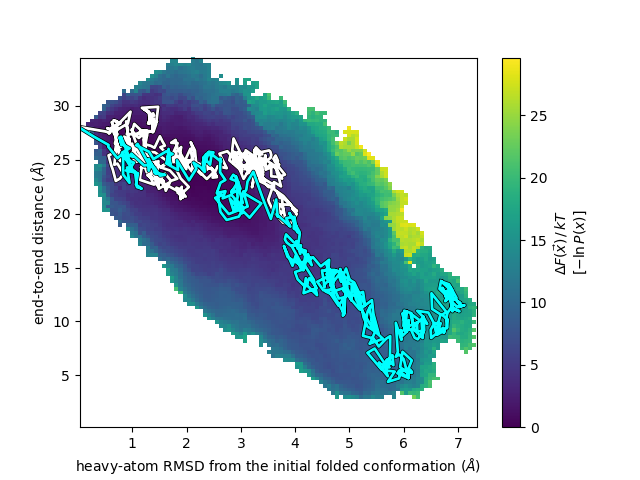
\includegraphics[width=\linewidth]{Figure13.png}
\caption{Two-dimensional probability distribution as a function of the progress coordinate. 
Two representative, continuous trajectories (435 and 279) that originate from distinct initial states are traced in cyan and white, respectively.}
\label{fig:view}
\end{figure}
%%%%%%%%

\section{Author Contributions}

AT Bogetti, B Mostofian, A Dickson, AJ Pratt, AS Saglam, PO Harrison, M Dudek, PA Torrillo, AJ DeGrave, and U Adhikari developed and wrote the tutorials; the primary author of each tutorial is designated as a co-first author of the overall manuscript and listed in the order in which the tutorials appear in the manuscript. LT Chong and DM Zuckerman provided guidance for tutorial development. 
AT Bogetti, LT Chong, DM Zuckerman, AJ Pratt, AS Saglam, B Mostofian, and MC Zwier wrote the introductory sections leading up to the tutorials. 

\section{Other Contributions}

We thank the many users of the WESTPA software who have provided important feedback for improving our tutorials and documentation over the past several years. We are also grateful to Samuel Lotz (Dickson Lab) for his contributions to the WESTPA-WExplore plugin.

\section{Potentially Conflicting Interests}

The authors declare no conflicting interests.

\section{Funding Information}

This work was supported by NIH R01 GM1151805-01 to LT Chong, DM Zuckerman, and MC Zwier; NSF CHE-1807301 and NIH R01 GM1115762 to LT Chong; a University of Pittsburgh Dietrich School of Arts and Sciences Graduate Fellowship to AT Bogetti; NIH R01GM130794 to A Dickson; NIH T32-DK061296 to JL Adelman; and a University of Pittsburgh Brackenridge Summer Undergraduate Fellowship to PA Torrillo.

\section{Content and links}

All files needed for the tutorials can be found at \url{https://github.com/westpa/westpa_tutorials}

\bibliography{TutorialsManuscript}

\newpage
\onecolumn
\begin{center}
\begin{LARGE}
    \textbf{PROTOCOL FOR RUNNING WE SIMULATIONS}
\end{LARGE}
\end{center}
\renewcommand{\theenumi}{\Roman{enumi}}
\renewcommand{\labelenumi}{\theenumi}
\renewcommand{\theenumii}{\arabic{enumii}}
\renewcommand{\labelenumii}{(\theenumii)}
\begin{enumerate}
\item Ready.
\begin{enumerate}
\item \textbf{Organize files into directories.} 
The initial coordinate file(s) should go in \verb|bstates| and the topology and MD input files should go in \verb|common_files|. 
In addition, any scripts needed to calculate the progress coordinate should be placed in \verb|common_files|. (p.12)
\item \textbf{Prepare the system environment.}  
Edit \verb|env.sh| accordingly for your system environment, i.e. source any files needed to set up the dynamics engine and set variables equal to the full paths of programs (see p. 12). 
\item \textbf{Specify WE parameters.}  
In the \verb|west.cfg| file, specify the number of WE iterations that will be carried out, progress coordinate, number of progress coordinate values that will be recorded per iteration, bin spacing, and number of trajectories per bin (see Section 3; Table 2).  
If a nested coordinate is desired, the bin spacing should be defined in \verb|system.py| (See point 4 on p. 8).  
The $\tau$ value is specified in the main input file for dynamics propagation (in \verb|common_files/|) through the total number of MD steps.  
If using the WExplore plugin, you will need to specify parameters that are unique to WExplore (see Section 3.1 and Tutorial 6.4).
\item \textbf{Set up calculations of auxiliary data.} 
Decide if you want to store any data that is auxiliary to the progress coordinate and add the corresponding datasets to \verb|west.cfg|.
\item \textbf{Specify whether to run equilibrium or steady-state WE.}
Edit the \verb|init.sh| file to include \verb|TSTATE_ARGS| if you plan to run steady-state WE.  
Also, edit \verb|tstate.file| to include the target state progress coordinate value(s). (p. 12) 
\item \textbf{Calculate your initial progress coordinate value(s).}
You can either set us this calculation manually, placing the contents in \textbf{pcoord.init} (see Basic Tutorial), or edit \verb|get_pcoord.sh| to calculate it (see Intermediate Tutorial) before those values are passed to WESTPA. (pp. 13-14)
\end{enumerate}
\item Set.
\begin{enumerate}
\item \textbf{Initialize the WE simulation.}  This is done by running \verb|init.sh|.
\item \textbf{Prepare to run the WE simulation.} Edit \verb|runseg.sh| to run dynamics, calculate the progress coordinate and store any auxiliary data. (p. 14)
\end{enumerate}
\item Go!
\begin{enumerate}
\item \textbf{Run the WE simulation.} 
To execute \verb|w_run| on your cluster, run an appropriate submission script (e.g., using Slurm).
\item \textbf{Monitor simulation progress.}
Backup your \verb|west.h5| file and use \verb|w_pdist| and \verb|plothist| to calculate and visualize probability distributions (pp. 14). 
If your WE simulation is not making any bin-to-bin transitions stop the simulation and restart the simulation with a shorter $\tau$, adjustments in the progress coordinate, and/or adjustments in bin spacings (pp. 16-17). 
\item \textbf{Assess simulation convergence.} 
Plot the average flux into the target state (or other observable of interest) as a function of WE iteration (p. 15).
\end{enumerate}
\item Analyze.
\begin{enumerate}
\item \textbf{Progress coordinate and auxiliary data.} 
Progress coordinate and auxiliary datasets are stored in the \verb|west.h5| file and can be extracted using \verb|hdfview| or the \verb|h5py| Python package. 
The \verb|w_ipa| tool can be used to calculate kinetic observables (e.g. rate constants), which are outputted to the \verb|assign.h5| and \verb|direct.h5 files|. (p. 15) 
To plot a dataset, use a plotting tool such as \verb|matplotlib|.
\item \textbf{Visualize a successful trajectory.}
Start by running \verb|w_succ| to obtain the WE iteration and segment of the final conformation from the successful trajectory (p. 14). 
Then, run \verb|w_trace| to obtain the series of conformations in the trajectory by tracing backwards from the final to initial conformations of the trajectory. 
The resulting series of conformations can then be visualized using a software package such as VMD. (p. 15) 
\end{enumerate}
\end{enumerate}

\newpage
\begin{center}
\begin{LARGE}
    \textbf{CHECKLIST FOR TROUBLESHOOTING WE SIMULATIONS}
\end{LARGE}
\end{center}

\renewcommand{\labelenumi}{}
\renewcommand{\labelenumii}{$\square$}
\begin{enumerate}
\item \textbf{Files for Dynamics Propagation}
\begin{enumerate}
\item Have you set up all of the files for propagating the dynamics using your dynamics engine (e.g. Amber, OpenMM)? 
\end{enumerate}
\item \textbf{System Configuration (}\verb|west.cfg| \textbf{file)}
\begin{enumerate}
\item Is \verb|pcoord_len| set to the number of data points that corresponds to the frequency with which the dynamics engine outputs the progress coordinate? Note: Many MD engines (e.g. Gromacs) output the initial point (i.e. zero). 
\item Are the bins in the expected positions? You can easily view the positions of the bins using a Python interpreter.
\end{enumerate}
\item \textbf{Initializing the simulation (}\verb|init.sh| \textbf{file)} 
\begin{enumerate}
\item Is the directory structure for the trajectory output files consistent with specifications in the \verb|west.cfg| file? 
\item Are the basis (\verb|bstate|) states, and if applicable, target states (\verb|tstate|), specified correctly?
\end{enumerate}
\item \textbf{Calculating the progress coordinate for initial states (}\verb|get_pcoord.sh| \textbf{file)}
\begin{enumerate}
\item Ensure that the procedure to extract the progress coordinate works by calculating your progress coordinate manually for one (or more) basis state files. 
\item Examine structure(s) of the initial states using visualization software (e.g. VMD, PyMOL) to verify that the structure(s) match the progress coordinate in the H5 file 
\end{enumerate}
\item \textbf{Segment implementation (}\verb|runseg.sh|\textbf{)}
\begin{enumerate}
\item Ensure that the progress coordinate is being calculated correctly by manually running a single dynamics segment of length $/tau$ for a single trajectory walker. 
Check that your analysis pipeline works using the output from the single dynamics segment. 
\item Are you feeding the information (e.g., coordinates, velocities) that is required for continuing trajectories? 
\item Check the \verb|seg_log| file to further ensure correct calculation of the progress coordinate. 
\item Ensure you are saving everything you might need to restart your simulation later on, including random seeds for stochastic dynamics as auxiliary data in the H5 file. 
\end{enumerate}
\item \textbf{Storage}
\begin{enumerate}
\item WESTPA simulations can generate a lot of data! Make sure you have enough space before starting the simulation.
\item Do you have a plan for backing up the simulation? 
Consider using tar to compress files from past iterations for easier backup. 
Keep file sizes =<300 GB. 
\item For all-atom explicit water simulations, it's a good idea to save a separate copy of your trajectories without water coordinates for more efficient analysis.
\end{enumerate}
\item \textbf{Simulation Progress (}\verb|west.h5| \textbf{file)}
\begin{enumerate}
\item Check that the first WE iteration has been initialized by typing \verb|h5ls west.h5/iterations| into the command line.  
You should see \verb|iter_00000001| in the output.
\item In addition, the progress coordinate should be initialized.
Check this by using the command 

\verb|h5ls -d west.h5/iterations/iter_00000001/pcoord|.
If all is well, the output will show that the array is populated by zeros and the first point is the value calculated by \verb|get_pcoord.sh|.
\end{enumerate}
\item \textbf{Analysis}
\begin{enumerate}
\item If you are running analysis on a shared computing resource, use the \verb|--serial| flag with the analysis tool. 
Otherwise, many of the included tools default to parallel mode (e.g., \verb|w_assign|), which will create as many Python threads as there are CPU cores available on your resource.
\end{enumerate}
\end{enumerate}

\end{document}
